% Chapter 11: Fractal markets hypothesis and long memory
% Statistics of Financial Markets -- Bachelor's programme, Bucharest University of Economic Studies
% GENERATED by latex/build_chapter11.py -- edit the generator, not this file.

\newcommand{\coursename}{Statistics of Financial Markets}
% Preambul comun SFM -- Statistica piețelor financiare / Statistics of Financial Markets (Beamer, 16:9)
% Același design ca MFM. Înainte de % Preambul comun SFM -- Statistica piețelor financiare / Statistics of Financial Markets (Beamer, 16:9)
% Același design ca MFM. Înainte de % Preambul comun SFM -- Statistica piețelor financiare / Statistics of Financial Markets (Beamer, 16:9)
% Același design ca MFM. Înainte de \input{../../latex/preamble} se definește
%   \newcommand{\coursename}{Statistics of Financial Markets}      (EN)
%   \newcommand{\coursename}{Statistica piețelor financiare}       (RO)  și  \def\sfmlang{ro}
% Fișierele .tex se află în EN/Courses, EN/Seminars, RO/Cursuri, RO/Seminarii (două niveluri sub rădăcină).
% Deck-urile sînt generate de latex/build_chapterN.py / build_seminarN.py (vezi latex/sfm_build.py).

\documentclass[9pt, aspectratio=169, t]{beamer}
\providecommand{\coursename}{Statistics of Financial Markets}

% Ensure content fits on slides
\setbeamersize{text margin left=8mm, text margin right=8mm}

%=============================================================================
% THEME AND STYLE CONFIGURATION
%=============================================================================
\usetheme{default}
% Using default theme for clean header/footer control

% Color Palette (matching Redispatch PDF)
\definecolor{MainBlue}{RGB}{26, 58, 110}
\definecolor{AccentBlue}{RGB}{26, 58, 110}
\definecolor{IDAred}{RGB}{205, 0, 0}
\definecolor{DarkGray}{RGB}{51, 51, 51}
\definecolor{MediumGray}{RGB}{128, 128, 128}
\definecolor{LightGray}{RGB}{248, 248, 248}
\definecolor{VeryLightGray}{RGB}{235, 235, 235}
\definecolor{KeynoteGray}{RGB}{218, 218, 218}
\definecolor{SectionGray}{RGB}{120, 120, 120}
\definecolor{FooterGray}{RGB}{100, 100, 100}
\definecolor{Crimson}{RGB}{220, 53, 69}
\definecolor{Forest}{RGB}{46, 125, 50}
\definecolor{Amber}{RGB}{181, 133, 63}
\definecolor{Orange}{RGB}{230, 126, 34}
\definecolor{Purple}{RGB}{142, 68, 173}

% Gradient background (exact Keynote 315° gradient: white to RGB 218,218,218)
\setbeamertemplate{background}{%
    \begin{tikzpicture}[remember picture, overlay]
        \shade[shading=axis, shading angle=315,
        top color=white, bottom color=KeynoteGray]
        (current page.south west) rectangle (current page.north east);
    \end{tikzpicture}%
}
% Fallback solid color for compatibility
\setbeamercolor{background canvas}{bg=}

\setbeamercolor{palette primary}{bg=MainBlue, fg=white}
\setbeamercolor{palette secondary}{bg=MainBlue!85, fg=white}
\setbeamercolor{palette tertiary}{bg=MainBlue!70, fg=white}
\setbeamercolor{structure}{fg=MainBlue}
\setbeamercolor{title}{fg=IDAred}
\setbeamercolor{frametitle}{fg=IDAred, bg=}
\setbeamercolor{block title}{bg=MainBlue, fg=white}
\setbeamercolor{block body}{bg=VeryLightGray, fg=DarkGray}
\setbeamercolor{block title alerted}{bg=Crimson, fg=white}
\setbeamercolor{block body alerted}{bg=Crimson!8, fg=DarkGray}
\setbeamercolor{block title example}{bg=Forest, fg=white}
\setbeamercolor{block body example}{bg=Forest!8, fg=DarkGray}
\setbeamercolor{item}{fg=MainBlue}

% Footer colors (override Madrid theme blue)
\setbeamercolor{author in head/foot}{fg=FooterGray, bg=}
\setbeamercolor{title in head/foot}{fg=FooterGray, bg=}
\setbeamercolor{date in head/foot}{fg=FooterGray, bg=}
\setbeamercolor{section in head/foot}{fg=FooterGray, bg=}
\setbeamercolor{subsection in head/foot}{fg=FooterGray, bg=}

% Bullet styles (apply everywhere including blocks)
\setbeamertemplate{itemize item}{\color{MainBlue}$\boxdot$}
\setbeamertemplate{itemize subitem}{\color{MainBlue}$\blacktriangleright$}
\setbeamertemplate{itemize subsubitem}{\color{MainBlue}\tiny$\bullet$}
\setbeamertemplate{itemize/enumerate body begin}{\normalsize}
\setbeamertemplate{itemize/enumerate subbody begin}{\normalsize}

% Item spacing - compact style
\setlength{\leftmargini}{10pt}       % Level 1: minimal indent
\setlength{\leftmarginii}{10pt}      % Level 2: minimal additional indent
% Compact list spacing (zero extra space before/after lists in blocks)
\makeatletter
\def\@listi{\leftmargin\leftmargini \topsep 0pt \parsep 0pt \itemsep 0pt}
\def\@listii{\leftmargin\leftmarginii \topsep 0pt \parsep 0pt \itemsep 0pt}
\makeatother

\setbeamertemplate{navigation symbols}{}

%=============================================================================
% CUSTOM HEADLINE
%=============================================================================
\setbeamertemplate{headline}{%
    \vskip10pt%
    \hbox to \paperwidth{%
        \hskip0.5cm%
        {\small\color{FooterGray}\renewcommand{\hyperlink}[2]{##2}\insertsectionhead}%
        \hfill%
        \textcolor{FooterGray}{\small\insertframenumber}%
        \hskip0.5cm%
    }%
    \vskip4pt%
    {\color{FooterGray}\hrule height 0.4pt}%
}

%=============================================================================
% CUSTOM FOOTER
%=============================================================================
\usepackage{fontawesome5}

\setbeamertemplate{footline}{%
    {\color{FooterGray}\hrule height 0.4pt}%
    \vskip4pt%
    \hbox to \paperwidth{%
        \hskip0.5cm%
        \textcolor{FooterGray}{\small\coursename}%
        \hfill%
        \raisebox{-0.1em}{%
            \begin{tikzpicture}[x=0.08em, y=0.08em, line width=0.4pt]
                \draw[FooterGray] (0,3) -- (1,4) -- (2,3.5) -- (3,5) -- (4,4) -- (5,6) -- (6,5.5) -- (7,4) -- (8,5) -- (9,7) -- (10,6) -- (11,5) -- (12,6.5) -- (13,8) -- (14,7) -- (15,6) -- (16,7.5) -- (17,9) -- (18,8) -- (19,7) -- (20,8.5) -- (21,10) -- (22,9) -- (23,8) -- (24,9.5);
            \end{tikzpicture}%
        }%
        \hskip0.5cm%
    }%
    \vskip6pt%
}

%=============================================================================
% PACKAGES
%=============================================================================
\usepackage[utf8]{inputenc}
\DeclareUnicodeCharacter{03B1}{\ensuremath{\alpha}}
\usepackage[T1]{fontenc}
\usepackage{amsmath, amssymb, amsthm}
\usepackage{mathtools}
\usepackage{bm}
\usepackage{tikz}
\usetikzlibrary{arrows.meta, positioning, shapes, calc, decorations.pathreplacing, shadings}
\usepackage{booktabs}
\usepackage{multirow}
\usepackage{array}
\usepackage{graphicx}
\usepackage{hyperref}
\usepackage{colortbl}
\usepackage{listings}
\lstset{language=Python, basicstyle=\ttfamily\scriptsize, keywordstyle=\color{MainBlue}\bfseries,
  commentstyle=\color{Forest}, stringstyle=\color{Crimson}, breaklines=true,
  frame=none, backgroundcolor=\color{VeryLightGray}, xleftmargin=2mm}
\hypersetup{colorlinks=true, linkcolor=MainBlue, urlcolor=MainBlue}
\graphicspath{{../../logos/}{../../charts/}{../../photos/}}
\usepackage{xcolor}
\hfuzz=2pt  % Suppress tiny overfull warnings (<2pt)
\vfuzz=2pt  % Suppress tiny vertical overfull warnings (<2pt)

%=============================================================================
% QUANTLET COMMANDS
%   \quantlet{<displayed name>}{<url>}       (generic, compatible with the older SFM decks)
%   \sfmquantlet{Ch_05}{SFM_ch5_garch}       -> https://github.com/danpele/SFM/tree/main/Quantlets/Ch_05/SFM_ch5_garch
%   \qlurl{<folder>} is defined per chapter by the generator (Quantlets/Ch_NN/<folder>)
%=============================================================================
\newcommand{\sfmrepo}{https://github.com/danpele/SFM}
\newcommand{\sfmqlbase}{https://github.com/danpele/SFM/tree/main/Quantlets}
\newcommand{\quantlet}[2]{%
    \hfill\href{#2}{%
        \raisebox{-0.15em}{
\includegraphics[height=0.7em]{ql_logo.png}}%
        \textcolor{MainBlue}{\tiny\ #1}%
    }%
}
\newcommand{\sfmquantlet}[2]{\quantlet{\detokenize{#2}}{\sfmqlbase/#1/#2}}

%=============================================================================
% NOTEBOOKS (Google Colab)
%   \colaburl{notebooks/EN/chapter5_seminar_notebook.ipynb} -> the Colab link of a file in the SFM repo
%   \nb: the chapter notebook (each seminar deck redefines it with \renewcommand)
%=============================================================================
\newcommand{\colaburl}[1]{https://colab.research.google.com/github/danpele/SFM/blob/main/#1}
\newcommand{\nb}{https://colab.research.google.com/github/danpele/SFM/tree/main/notebooks/EN}
\newcommand{\nbname}{notebooks/EN}

%=============================================================================
% SLIDE HELPERS (used by the generators; the same as in MFM)
%=============================================================================
% local font size for list bodies (the preamble forces \normalsize)
\newcommand{\itemsize}[1]{\setbeamertemplate{itemize/enumerate body begin}{#1}\setbeamertemplate{itemize/enumerate subbody begin}{#1}}
\newcommand{\intitle}[1]{{\hypersetup{urlcolor=white}#1}}   % white links inside coloured title bars
\newcommand{\imgcap}[1]{{\scriptsize #1}\\[0.5mm]}          % caption under a photo
\newcommand{\imgcredit}[2]{{\tiny\color{FooterGray}\href{#1}{#2}}}   % image credit: source URL, author/licence
\newcommand{\aiprompt}[1]{{\ttfamily\color{MainBlue}#1}}     % a prompt to an AI assistant

%=============================================================================
% SEMINARS: student version by default; the instructor wrapper *_solutions.tex sets \solutionstrue
%=============================================================================
\makeatletter\@ifundefined{ifsolutions}{\expandafter\newif\csname ifsolutions\endcsname}{}\makeatother
\newcommand{\solonly}[1]{\ifsolutions #1\fi}
\newcommand{\propsub}{\ifsolutions\else\framesubtitle{\ifdefined\sfmlang Rezolvarea se discută la seminar\else Solution discussed in class\fi}\fi}

%=============================================================================
% APPENDIX AND CHAPTER LINKS (latex/appendix_links.py writes the calls; it also re-declares these
% macros before \begin{document}, so the decks compile with or without this preamble block)
%=============================================================================
\providecommand{\sfmapplink}[3]{\hypertarget{#2}{}\hyperlink{#1}{\beamergotobutton{#3}}}
\providecommand{\sfmappback}[2]{\begin{tikzpicture}[remember picture,overlay]\node[anchor=south east] at ([xshift=-3mm,yshift=7mm]current page.south east){\hyperlink{#1}{\beamerreturnbutton{#2}}};\end{tikzpicture}}
\providecommand{\sfmchlink}[2]{\href{#1}{#2}}
\providecommand{\sfmchlinkt}[2]{\href{#1}{\usebeamercolor[fg]{frametitle}#2}}

%=============================================================================
% QUANTINAR COMMAND: link către un curs Quantinar (subiecte avansate)
%=============================================================================
\newcommand{\quantinar}[2]{%
    \href{#2}{%
        \raisebox{-0.15em}{
\includegraphics[height=0.8em]{qr_logo.png}}%
        \textcolor{MainBlue}{\scriptsize\ #1}%
    }%
}

%=============================================================================
% CUSTOM TITLE PAGE
%=============================================================================
\defbeamertemplate*{title page}{hybrid}[1][]
{
    \vspace{0.2cm}
    % Logos row - top header (with clickable links)
    \begin{center}
        \href{https://www.ase.ro}{
\includegraphics[height=1.0cm]{ase_logo.png}}\hspace{0.3cm}%
        \href{https://theida.net}{
\includegraphics[height=1.0cm]{ida_logo.png}}\hspace{0.3cm}%
        \href{https://blockchain-research-center.com}{
\includegraphics[height=1.0cm]{brc_logo.png}}\hspace{0.3cm}%
        \href{https://www.ai4efin.ase.ro}{
\includegraphics[height=1.0cm]{ai4efin_logo.png}}\hspace{0.3cm}%
        \href{https://ipe.ro/new}{
\includegraphics[height=1.0cm]{acad_logo.png}}\hspace{0.3cm}%
        \href{https://www.digital-finance-msca.com}{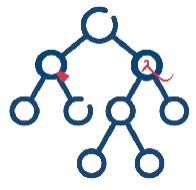
\includegraphics[height=1.0cm]{msca_logo.png}}%
    \end{center}

    \vspace{0.6cm}

    % Main title with Q logos on sides (with clickable links)
    \begin{center}
        \begin{minipage}{0.1\textwidth}
            \centering
            \href{https://quantlet.com}{
\includegraphics[height=1.1cm]{ql_logo.png}}
        \end{minipage}%
        \begin{minipage}{0.78\textwidth}
            \centering
            {\LARGE\bfseries\usebeamercolor[fg]{title}\inserttitle}

            \vspace{0.3cm}

            {\usebeamerfont{subtitle}\usebeamercolor[fg]{title}\insertsubtitle}
        \end{minipage}%
        \begin{minipage}{0.1\textwidth}
            \centering
            \href{https://quantinar.com}{
\includegraphics[height=1.1cm]{qr_logo.png}}
        \end{minipage}
    \end{center}

    \vspace{0.6cm}

    % Authors (left aligned)
    \hspace{0.5cm}{\usebeamerfont{author}\insertauthor}

    \vspace{0.3cm}

    % Institute/Affiliations (left aligned)
    \hspace{0.5cm}\begin{minipage}[t]{0.9\textwidth}
        \raggedright\small\insertinstitute
    \end{minipage}
}

%=============================================================================
% THEOREM ENVIRONMENTS
%=============================================================================
\theoremstyle{definition}
\setbeamertemplate{theorems}[numbered]
\ifdefined\sfmlang
\newtheorem{defn}{Definiție}
\newtheorem{thm}{Teoremă}
\newtheorem{prop}{Propoziție}
\newtheorem{rmk}{Observație}
\else
\newtheorem{defn}{Definition}
\newtheorem{thm}{Theorem}
\newtheorem{prop}{Proposition}
\newtheorem{rmk}{Remark}
\fi

%=============================================================================
% CENTRED MINIPAGE (no extra vertical space)
%=============================================================================
\newenvironment{cminipage}[1]{%
    \par\noindent\hfill\begin{minipage}{#1}\ignorespaces
}{%
    \end{minipage}\hfill\null\par
}

%=============================================================================
% CUSTOM COMMANDS
%=============================================================================
\newcommand{\E}{\mathbb{E}}
\newcommand{\Var}{\text{Var}}
\newcommand{\Cov}{\text{Cov}}
\newcommand{\Corr}{\text{Corr}}
\newcommand{\R}{\mathbb{R}}
\newcommand{\N}{\mathbb{N}}
\newcommand{\Z}{\mathbb{Z}}
\newcommand{\B}{\mathbf{B}}
\newcommand{\imark}{\textcolor{MainBlue}{\textbullet}}
\newcommand{\RMSE}{\text{RMSE}}
\newcommand{\MAE}{\text{MAE}}
\newcommand{\MAPE}{\text{MAPE}}

 se definește
%   \newcommand{\coursename}{Statistics of Financial Markets}      (EN)
%   \newcommand{\coursename}{Statistica piețelor financiare}       (RO)  și  \def\sfmlang{ro}
% Fișierele .tex se află în EN/Courses, EN/Seminars, RO/Cursuri, RO/Seminarii (două niveluri sub rădăcină).
% Deck-urile sînt generate de latex/build_chapterN.py / build_seminarN.py (vezi latex/sfm_build.py).

\documentclass[9pt, aspectratio=169, t]{beamer}
\providecommand{\coursename}{Statistics of Financial Markets}

% Ensure content fits on slides
\setbeamersize{text margin left=8mm, text margin right=8mm}

%=============================================================================
% THEME AND STYLE CONFIGURATION
%=============================================================================
\usetheme{default}
% Using default theme for clean header/footer control

% Color Palette (matching Redispatch PDF)
\definecolor{MainBlue}{RGB}{26, 58, 110}
\definecolor{AccentBlue}{RGB}{26, 58, 110}
\definecolor{IDAred}{RGB}{205, 0, 0}
\definecolor{DarkGray}{RGB}{51, 51, 51}
\definecolor{MediumGray}{RGB}{128, 128, 128}
\definecolor{LightGray}{RGB}{248, 248, 248}
\definecolor{VeryLightGray}{RGB}{235, 235, 235}
\definecolor{KeynoteGray}{RGB}{218, 218, 218}
\definecolor{SectionGray}{RGB}{120, 120, 120}
\definecolor{FooterGray}{RGB}{100, 100, 100}
\definecolor{Crimson}{RGB}{220, 53, 69}
\definecolor{Forest}{RGB}{46, 125, 50}
\definecolor{Amber}{RGB}{181, 133, 63}
\definecolor{Orange}{RGB}{230, 126, 34}
\definecolor{Purple}{RGB}{142, 68, 173}

% Gradient background (exact Keynote 315° gradient: white to RGB 218,218,218)
\setbeamertemplate{background}{%
    \begin{tikzpicture}[remember picture, overlay]
        \shade[shading=axis, shading angle=315,
        top color=white, bottom color=KeynoteGray]
        (current page.south west) rectangle (current page.north east);
    \end{tikzpicture}%
}
% Fallback solid color for compatibility
\setbeamercolor{background canvas}{bg=}

\setbeamercolor{palette primary}{bg=MainBlue, fg=white}
\setbeamercolor{palette secondary}{bg=MainBlue!85, fg=white}
\setbeamercolor{palette tertiary}{bg=MainBlue!70, fg=white}
\setbeamercolor{structure}{fg=MainBlue}
\setbeamercolor{title}{fg=IDAred}
\setbeamercolor{frametitle}{fg=IDAred, bg=}
\setbeamercolor{block title}{bg=MainBlue, fg=white}
\setbeamercolor{block body}{bg=VeryLightGray, fg=DarkGray}
\setbeamercolor{block title alerted}{bg=Crimson, fg=white}
\setbeamercolor{block body alerted}{bg=Crimson!8, fg=DarkGray}
\setbeamercolor{block title example}{bg=Forest, fg=white}
\setbeamercolor{block body example}{bg=Forest!8, fg=DarkGray}
\setbeamercolor{item}{fg=MainBlue}

% Footer colors (override Madrid theme blue)
\setbeamercolor{author in head/foot}{fg=FooterGray, bg=}
\setbeamercolor{title in head/foot}{fg=FooterGray, bg=}
\setbeamercolor{date in head/foot}{fg=FooterGray, bg=}
\setbeamercolor{section in head/foot}{fg=FooterGray, bg=}
\setbeamercolor{subsection in head/foot}{fg=FooterGray, bg=}

% Bullet styles (apply everywhere including blocks)
\setbeamertemplate{itemize item}{\color{MainBlue}$\boxdot$}
\setbeamertemplate{itemize subitem}{\color{MainBlue}$\blacktriangleright$}
\setbeamertemplate{itemize subsubitem}{\color{MainBlue}\tiny$\bullet$}
\setbeamertemplate{itemize/enumerate body begin}{\normalsize}
\setbeamertemplate{itemize/enumerate subbody begin}{\normalsize}

% Item spacing - compact style
\setlength{\leftmargini}{10pt}       % Level 1: minimal indent
\setlength{\leftmarginii}{10pt}      % Level 2: minimal additional indent
% Compact list spacing (zero extra space before/after lists in blocks)
\makeatletter
\def\@listi{\leftmargin\leftmargini \topsep 0pt \parsep 0pt \itemsep 0pt}
\def\@listii{\leftmargin\leftmarginii \topsep 0pt \parsep 0pt \itemsep 0pt}
\makeatother

\setbeamertemplate{navigation symbols}{}

%=============================================================================
% CUSTOM HEADLINE
%=============================================================================
\setbeamertemplate{headline}{%
    \vskip10pt%
    \hbox to \paperwidth{%
        \hskip0.5cm%
        {\small\color{FooterGray}\renewcommand{\hyperlink}[2]{##2}\insertsectionhead}%
        \hfill%
        \textcolor{FooterGray}{\small\insertframenumber}%
        \hskip0.5cm%
    }%
    \vskip4pt%
    {\color{FooterGray}\hrule height 0.4pt}%
}

%=============================================================================
% CUSTOM FOOTER
%=============================================================================
\usepackage{fontawesome5}

\setbeamertemplate{footline}{%
    {\color{FooterGray}\hrule height 0.4pt}%
    \vskip4pt%
    \hbox to \paperwidth{%
        \hskip0.5cm%
        \textcolor{FooterGray}{\small\coursename}%
        \hfill%
        \raisebox{-0.1em}{%
            \begin{tikzpicture}[x=0.08em, y=0.08em, line width=0.4pt]
                \draw[FooterGray] (0,3) -- (1,4) -- (2,3.5) -- (3,5) -- (4,4) -- (5,6) -- (6,5.5) -- (7,4) -- (8,5) -- (9,7) -- (10,6) -- (11,5) -- (12,6.5) -- (13,8) -- (14,7) -- (15,6) -- (16,7.5) -- (17,9) -- (18,8) -- (19,7) -- (20,8.5) -- (21,10) -- (22,9) -- (23,8) -- (24,9.5);
            \end{tikzpicture}%
        }%
        \hskip0.5cm%
    }%
    \vskip6pt%
}

%=============================================================================
% PACKAGES
%=============================================================================
\usepackage[utf8]{inputenc}
\DeclareUnicodeCharacter{03B1}{\ensuremath{\alpha}}
\usepackage[T1]{fontenc}
\usepackage{amsmath, amssymb, amsthm}
\usepackage{mathtools}
\usepackage{bm}
\usepackage{tikz}
\usetikzlibrary{arrows.meta, positioning, shapes, calc, decorations.pathreplacing, shadings}
\usepackage{booktabs}
\usepackage{multirow}
\usepackage{array}
\usepackage{graphicx}
\usepackage{hyperref}
\usepackage{colortbl}
\usepackage{listings}
\lstset{language=Python, basicstyle=\ttfamily\scriptsize, keywordstyle=\color{MainBlue}\bfseries,
  commentstyle=\color{Forest}, stringstyle=\color{Crimson}, breaklines=true,
  frame=none, backgroundcolor=\color{VeryLightGray}, xleftmargin=2mm}
\hypersetup{colorlinks=true, linkcolor=MainBlue, urlcolor=MainBlue}
\graphicspath{{../../logos/}{../../charts/}{../../photos/}}
\usepackage{xcolor}
\hfuzz=2pt  % Suppress tiny overfull warnings (<2pt)
\vfuzz=2pt  % Suppress tiny vertical overfull warnings (<2pt)

%=============================================================================
% QUANTLET COMMANDS
%   \quantlet{<displayed name>}{<url>}       (generic, compatible with the older SFM decks)
%   \sfmquantlet{Ch_05}{SFM_ch5_garch}       -> https://github.com/danpele/SFM/tree/main/Quantlets/Ch_05/SFM_ch5_garch
%   \qlurl{<folder>} is defined per chapter by the generator (Quantlets/Ch_NN/<folder>)
%=============================================================================
\newcommand{\sfmrepo}{https://github.com/danpele/SFM}
\newcommand{\sfmqlbase}{https://github.com/danpele/SFM/tree/main/Quantlets}
\newcommand{\quantlet}[2]{%
    \hfill\href{#2}{%
        \raisebox{-0.15em}{
\includegraphics[height=0.7em]{ql_logo.png}}%
        \textcolor{MainBlue}{\tiny\ #1}%
    }%
}
\newcommand{\sfmquantlet}[2]{\quantlet{\detokenize{#2}}{\sfmqlbase/#1/#2}}

%=============================================================================
% NOTEBOOKS (Google Colab)
%   \colaburl{notebooks/EN/chapter5_seminar_notebook.ipynb} -> the Colab link of a file in the SFM repo
%   \nb: the chapter notebook (each seminar deck redefines it with \renewcommand)
%=============================================================================
\newcommand{\colaburl}[1]{https://colab.research.google.com/github/danpele/SFM/blob/main/#1}
\newcommand{\nb}{https://colab.research.google.com/github/danpele/SFM/tree/main/notebooks/EN}
\newcommand{\nbname}{notebooks/EN}

%=============================================================================
% SLIDE HELPERS (used by the generators; the same as in MFM)
%=============================================================================
% local font size for list bodies (the preamble forces \normalsize)
\newcommand{\itemsize}[1]{\setbeamertemplate{itemize/enumerate body begin}{#1}\setbeamertemplate{itemize/enumerate subbody begin}{#1}}
\newcommand{\intitle}[1]{{\hypersetup{urlcolor=white}#1}}   % white links inside coloured title bars
\newcommand{\imgcap}[1]{{\scriptsize #1}\\[0.5mm]}          % caption under a photo
\newcommand{\imgcredit}[2]{{\tiny\color{FooterGray}\href{#1}{#2}}}   % image credit: source URL, author/licence
\newcommand{\aiprompt}[1]{{\ttfamily\color{MainBlue}#1}}     % a prompt to an AI assistant

%=============================================================================
% SEMINARS: student version by default; the instructor wrapper *_solutions.tex sets \solutionstrue
%=============================================================================
\makeatletter\@ifundefined{ifsolutions}{\expandafter\newif\csname ifsolutions\endcsname}{}\makeatother
\newcommand{\solonly}[1]{\ifsolutions #1\fi}
\newcommand{\propsub}{\ifsolutions\else\framesubtitle{\ifdefined\sfmlang Rezolvarea se discută la seminar\else Solution discussed in class\fi}\fi}

%=============================================================================
% APPENDIX AND CHAPTER LINKS (latex/appendix_links.py writes the calls; it also re-declares these
% macros before \begin{document}, so the decks compile with or without this preamble block)
%=============================================================================
\providecommand{\sfmapplink}[3]{\hypertarget{#2}{}\hyperlink{#1}{\beamergotobutton{#3}}}
\providecommand{\sfmappback}[2]{\begin{tikzpicture}[remember picture,overlay]\node[anchor=south east] at ([xshift=-3mm,yshift=7mm]current page.south east){\hyperlink{#1}{\beamerreturnbutton{#2}}};\end{tikzpicture}}
\providecommand{\sfmchlink}[2]{\href{#1}{#2}}
\providecommand{\sfmchlinkt}[2]{\href{#1}{\usebeamercolor[fg]{frametitle}#2}}

%=============================================================================
% QUANTINAR COMMAND: link către un curs Quantinar (subiecte avansate)
%=============================================================================
\newcommand{\quantinar}[2]{%
    \href{#2}{%
        \raisebox{-0.15em}{
\includegraphics[height=0.8em]{qr_logo.png}}%
        \textcolor{MainBlue}{\scriptsize\ #1}%
    }%
}

%=============================================================================
% CUSTOM TITLE PAGE
%=============================================================================
\defbeamertemplate*{title page}{hybrid}[1][]
{
    \vspace{0.2cm}
    % Logos row - top header (with clickable links)
    \begin{center}
        \href{https://www.ase.ro}{
\includegraphics[height=1.0cm]{ase_logo.png}}\hspace{0.3cm}%
        \href{https://theida.net}{
\includegraphics[height=1.0cm]{ida_logo.png}}\hspace{0.3cm}%
        \href{https://blockchain-research-center.com}{
\includegraphics[height=1.0cm]{brc_logo.png}}\hspace{0.3cm}%
        \href{https://www.ai4efin.ase.ro}{
\includegraphics[height=1.0cm]{ai4efin_logo.png}}\hspace{0.3cm}%
        \href{https://ipe.ro/new}{
\includegraphics[height=1.0cm]{acad_logo.png}}\hspace{0.3cm}%
        \href{https://www.digital-finance-msca.com}{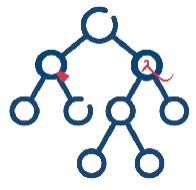
\includegraphics[height=1.0cm]{msca_logo.png}}%
    \end{center}

    \vspace{0.6cm}

    % Main title with Q logos on sides (with clickable links)
    \begin{center}
        \begin{minipage}{0.1\textwidth}
            \centering
            \href{https://quantlet.com}{
\includegraphics[height=1.1cm]{ql_logo.png}}
        \end{minipage}%
        \begin{minipage}{0.78\textwidth}
            \centering
            {\LARGE\bfseries\usebeamercolor[fg]{title}\inserttitle}

            \vspace{0.3cm}

            {\usebeamerfont{subtitle}\usebeamercolor[fg]{title}\insertsubtitle}
        \end{minipage}%
        \begin{minipage}{0.1\textwidth}
            \centering
            \href{https://quantinar.com}{
\includegraphics[height=1.1cm]{qr_logo.png}}
        \end{minipage}
    \end{center}

    \vspace{0.6cm}

    % Authors (left aligned)
    \hspace{0.5cm}{\usebeamerfont{author}\insertauthor}

    \vspace{0.3cm}

    % Institute/Affiliations (left aligned)
    \hspace{0.5cm}\begin{minipage}[t]{0.9\textwidth}
        \raggedright\small\insertinstitute
    \end{minipage}
}

%=============================================================================
% THEOREM ENVIRONMENTS
%=============================================================================
\theoremstyle{definition}
\setbeamertemplate{theorems}[numbered]
\ifdefined\sfmlang
\newtheorem{defn}{Definiție}
\newtheorem{thm}{Teoremă}
\newtheorem{prop}{Propoziție}
\newtheorem{rmk}{Observație}
\else
\newtheorem{defn}{Definition}
\newtheorem{thm}{Theorem}
\newtheorem{prop}{Proposition}
\newtheorem{rmk}{Remark}
\fi

%=============================================================================
% CENTRED MINIPAGE (no extra vertical space)
%=============================================================================
\newenvironment{cminipage}[1]{%
    \par\noindent\hfill\begin{minipage}{#1}\ignorespaces
}{%
    \end{minipage}\hfill\null\par
}

%=============================================================================
% CUSTOM COMMANDS
%=============================================================================
\newcommand{\E}{\mathbb{E}}
\newcommand{\Var}{\text{Var}}
\newcommand{\Cov}{\text{Cov}}
\newcommand{\Corr}{\text{Corr}}
\newcommand{\R}{\mathbb{R}}
\newcommand{\N}{\mathbb{N}}
\newcommand{\Z}{\mathbb{Z}}
\newcommand{\B}{\mathbf{B}}
\newcommand{\imark}{\textcolor{MainBlue}{\textbullet}}
\newcommand{\RMSE}{\text{RMSE}}
\newcommand{\MAE}{\text{MAE}}
\newcommand{\MAPE}{\text{MAPE}}

 se definește
%   \newcommand{\coursename}{Statistics of Financial Markets}      (EN)
%   \newcommand{\coursename}{Statistica piețelor financiare}       (RO)  și  \def\sfmlang{ro}
% Fișierele .tex se află în EN/Courses, EN/Seminars, RO/Cursuri, RO/Seminarii (două niveluri sub rădăcină).
% Deck-urile sînt generate de latex/build_chapterN.py / build_seminarN.py (vezi latex/sfm_build.py).

\documentclass[9pt, aspectratio=169, t]{beamer}
\providecommand{\coursename}{Statistics of Financial Markets}

% Ensure content fits on slides
\setbeamersize{text margin left=8mm, text margin right=8mm}

%=============================================================================
% THEME AND STYLE CONFIGURATION
%=============================================================================
\usetheme{default}
% Using default theme for clean header/footer control

% Color Palette (matching Redispatch PDF)
\definecolor{MainBlue}{RGB}{26, 58, 110}
\definecolor{AccentBlue}{RGB}{26, 58, 110}
\definecolor{IDAred}{RGB}{205, 0, 0}
\definecolor{DarkGray}{RGB}{51, 51, 51}
\definecolor{MediumGray}{RGB}{128, 128, 128}
\definecolor{LightGray}{RGB}{248, 248, 248}
\definecolor{VeryLightGray}{RGB}{235, 235, 235}
\definecolor{KeynoteGray}{RGB}{218, 218, 218}
\definecolor{SectionGray}{RGB}{120, 120, 120}
\definecolor{FooterGray}{RGB}{100, 100, 100}
\definecolor{Crimson}{RGB}{220, 53, 69}
\definecolor{Forest}{RGB}{46, 125, 50}
\definecolor{Amber}{RGB}{181, 133, 63}
\definecolor{Orange}{RGB}{230, 126, 34}
\definecolor{Purple}{RGB}{142, 68, 173}

% Gradient background (exact Keynote 315° gradient: white to RGB 218,218,218)
\setbeamertemplate{background}{%
    \begin{tikzpicture}[remember picture, overlay]
        \shade[shading=axis, shading angle=315,
        top color=white, bottom color=KeynoteGray]
        (current page.south west) rectangle (current page.north east);
    \end{tikzpicture}%
}
% Fallback solid color for compatibility
\setbeamercolor{background canvas}{bg=}

\setbeamercolor{palette primary}{bg=MainBlue, fg=white}
\setbeamercolor{palette secondary}{bg=MainBlue!85, fg=white}
\setbeamercolor{palette tertiary}{bg=MainBlue!70, fg=white}
\setbeamercolor{structure}{fg=MainBlue}
\setbeamercolor{title}{fg=IDAred}
\setbeamercolor{frametitle}{fg=IDAred, bg=}
\setbeamercolor{block title}{bg=MainBlue, fg=white}
\setbeamercolor{block body}{bg=VeryLightGray, fg=DarkGray}
\setbeamercolor{block title alerted}{bg=Crimson, fg=white}
\setbeamercolor{block body alerted}{bg=Crimson!8, fg=DarkGray}
\setbeamercolor{block title example}{bg=Forest, fg=white}
\setbeamercolor{block body example}{bg=Forest!8, fg=DarkGray}
\setbeamercolor{item}{fg=MainBlue}

% Footer colors (override Madrid theme blue)
\setbeamercolor{author in head/foot}{fg=FooterGray, bg=}
\setbeamercolor{title in head/foot}{fg=FooterGray, bg=}
\setbeamercolor{date in head/foot}{fg=FooterGray, bg=}
\setbeamercolor{section in head/foot}{fg=FooterGray, bg=}
\setbeamercolor{subsection in head/foot}{fg=FooterGray, bg=}

% Bullet styles (apply everywhere including blocks)
\setbeamertemplate{itemize item}{\color{MainBlue}$\boxdot$}
\setbeamertemplate{itemize subitem}{\color{MainBlue}$\blacktriangleright$}
\setbeamertemplate{itemize subsubitem}{\color{MainBlue}\tiny$\bullet$}
\setbeamertemplate{itemize/enumerate body begin}{\normalsize}
\setbeamertemplate{itemize/enumerate subbody begin}{\normalsize}

% Item spacing - compact style
\setlength{\leftmargini}{10pt}       % Level 1: minimal indent
\setlength{\leftmarginii}{10pt}      % Level 2: minimal additional indent
% Compact list spacing (zero extra space before/after lists in blocks)
\makeatletter
\def\@listi{\leftmargin\leftmargini \topsep 0pt \parsep 0pt \itemsep 0pt}
\def\@listii{\leftmargin\leftmarginii \topsep 0pt \parsep 0pt \itemsep 0pt}
\makeatother

\setbeamertemplate{navigation symbols}{}

%=============================================================================
% CUSTOM HEADLINE
%=============================================================================
\setbeamertemplate{headline}{%
    \vskip10pt%
    \hbox to \paperwidth{%
        \hskip0.5cm%
        {\small\color{FooterGray}\renewcommand{\hyperlink}[2]{##2}\insertsectionhead}%
        \hfill%
        \textcolor{FooterGray}{\small\insertframenumber}%
        \hskip0.5cm%
    }%
    \vskip4pt%
    {\color{FooterGray}\hrule height 0.4pt}%
}

%=============================================================================
% CUSTOM FOOTER
%=============================================================================
\usepackage{fontawesome5}

\setbeamertemplate{footline}{%
    {\color{FooterGray}\hrule height 0.4pt}%
    \vskip4pt%
    \hbox to \paperwidth{%
        \hskip0.5cm%
        \textcolor{FooterGray}{\small\coursename}%
        \hfill%
        \raisebox{-0.1em}{%
            \begin{tikzpicture}[x=0.08em, y=0.08em, line width=0.4pt]
                \draw[FooterGray] (0,3) -- (1,4) -- (2,3.5) -- (3,5) -- (4,4) -- (5,6) -- (6,5.5) -- (7,4) -- (8,5) -- (9,7) -- (10,6) -- (11,5) -- (12,6.5) -- (13,8) -- (14,7) -- (15,6) -- (16,7.5) -- (17,9) -- (18,8) -- (19,7) -- (20,8.5) -- (21,10) -- (22,9) -- (23,8) -- (24,9.5);
            \end{tikzpicture}%
        }%
        \hskip0.5cm%
    }%
    \vskip6pt%
}

%=============================================================================
% PACKAGES
%=============================================================================
\usepackage[utf8]{inputenc}
\DeclareUnicodeCharacter{03B1}{\ensuremath{\alpha}}
\usepackage[T1]{fontenc}
\usepackage{amsmath, amssymb, amsthm}
\usepackage{mathtools}
\usepackage{bm}
\usepackage{tikz}
\usetikzlibrary{arrows.meta, positioning, shapes, calc, decorations.pathreplacing, shadings}
\usepackage{booktabs}
\usepackage{multirow}
\usepackage{array}
\usepackage{graphicx}
\usepackage{hyperref}
\usepackage{colortbl}
\usepackage{listings}
\lstset{language=Python, basicstyle=\ttfamily\scriptsize, keywordstyle=\color{MainBlue}\bfseries,
  commentstyle=\color{Forest}, stringstyle=\color{Crimson}, breaklines=true,
  frame=none, backgroundcolor=\color{VeryLightGray}, xleftmargin=2mm}
\hypersetup{colorlinks=true, linkcolor=MainBlue, urlcolor=MainBlue}
\graphicspath{{../../logos/}{../../charts/}{../../photos/}}
\usepackage{xcolor}
\hfuzz=2pt  % Suppress tiny overfull warnings (<2pt)
\vfuzz=2pt  % Suppress tiny vertical overfull warnings (<2pt)

%=============================================================================
% QUANTLET COMMANDS
%   \quantlet{<displayed name>}{<url>}       (generic, compatible with the older SFM decks)
%   \sfmquantlet{Ch_05}{SFM_ch5_garch}       -> https://github.com/danpele/SFM/tree/main/Quantlets/Ch_05/SFM_ch5_garch
%   \qlurl{<folder>} is defined per chapter by the generator (Quantlets/Ch_NN/<folder>)
%=============================================================================
\newcommand{\sfmrepo}{https://github.com/danpele/SFM}
\newcommand{\sfmqlbase}{https://github.com/danpele/SFM/tree/main/Quantlets}
\newcommand{\quantlet}[2]{%
    \hfill\href{#2}{%
        \raisebox{-0.15em}{
\includegraphics[height=0.7em]{ql_logo.png}}%
        \textcolor{MainBlue}{\tiny\ #1}%
    }%
}
\newcommand{\sfmquantlet}[2]{\quantlet{\detokenize{#2}}{\sfmqlbase/#1/#2}}

%=============================================================================
% NOTEBOOKS (Google Colab)
%   \colaburl{notebooks/EN/chapter5_seminar_notebook.ipynb} -> the Colab link of a file in the SFM repo
%   \nb: the chapter notebook (each seminar deck redefines it with \renewcommand)
%=============================================================================
\newcommand{\colaburl}[1]{https://colab.research.google.com/github/danpele/SFM/blob/main/#1}
\newcommand{\nb}{https://colab.research.google.com/github/danpele/SFM/tree/main/notebooks/EN}
\newcommand{\nbname}{notebooks/EN}

%=============================================================================
% SLIDE HELPERS (used by the generators; the same as in MFM)
%=============================================================================
% local font size for list bodies (the preamble forces \normalsize)
\newcommand{\itemsize}[1]{\setbeamertemplate{itemize/enumerate body begin}{#1}\setbeamertemplate{itemize/enumerate subbody begin}{#1}}
\newcommand{\intitle}[1]{{\hypersetup{urlcolor=white}#1}}   % white links inside coloured title bars
\newcommand{\imgcap}[1]{{\scriptsize #1}\\[0.5mm]}          % caption under a photo
\newcommand{\imgcredit}[2]{{\tiny\color{FooterGray}\href{#1}{#2}}}   % image credit: source URL, author/licence
\newcommand{\aiprompt}[1]{{\ttfamily\color{MainBlue}#1}}     % a prompt to an AI assistant

%=============================================================================
% SEMINARS: student version by default; the instructor wrapper *_solutions.tex sets \solutionstrue
%=============================================================================
\makeatletter\@ifundefined{ifsolutions}{\expandafter\newif\csname ifsolutions\endcsname}{}\makeatother
\newcommand{\solonly}[1]{\ifsolutions #1\fi}
\newcommand{\propsub}{\ifsolutions\else\framesubtitle{\ifdefined\sfmlang Rezolvarea se discută la seminar\else Solution discussed in class\fi}\fi}

%=============================================================================
% APPENDIX AND CHAPTER LINKS (latex/appendix_links.py writes the calls; it also re-declares these
% macros before \begin{document}, so the decks compile with or without this preamble block)
%=============================================================================
\providecommand{\sfmapplink}[3]{\hypertarget{#2}{}\hyperlink{#1}{\beamergotobutton{#3}}}
\providecommand{\sfmappback}[2]{\begin{tikzpicture}[remember picture,overlay]\node[anchor=south east] at ([xshift=-3mm,yshift=7mm]current page.south east){\hyperlink{#1}{\beamerreturnbutton{#2}}};\end{tikzpicture}}
\providecommand{\sfmchlink}[2]{\href{#1}{#2}}
\providecommand{\sfmchlinkt}[2]{\href{#1}{\usebeamercolor[fg]{frametitle}#2}}

%=============================================================================
% QUANTINAR COMMAND: link către un curs Quantinar (subiecte avansate)
%=============================================================================
\newcommand{\quantinar}[2]{%
    \href{#2}{%
        \raisebox{-0.15em}{
\includegraphics[height=0.8em]{qr_logo.png}}%
        \textcolor{MainBlue}{\scriptsize\ #1}%
    }%
}

%=============================================================================
% CUSTOM TITLE PAGE
%=============================================================================
\defbeamertemplate*{title page}{hybrid}[1][]
{
    \vspace{0.2cm}
    % Logos row - top header (with clickable links)
    \begin{center}
        \href{https://www.ase.ro}{
\includegraphics[height=1.0cm]{ase_logo.png}}\hspace{0.3cm}%
        \href{https://theida.net}{
\includegraphics[height=1.0cm]{ida_logo.png}}\hspace{0.3cm}%
        \href{https://blockchain-research-center.com}{
\includegraphics[height=1.0cm]{brc_logo.png}}\hspace{0.3cm}%
        \href{https://www.ai4efin.ase.ro}{
\includegraphics[height=1.0cm]{ai4efin_logo.png}}\hspace{0.3cm}%
        \href{https://ipe.ro/new}{
\includegraphics[height=1.0cm]{acad_logo.png}}\hspace{0.3cm}%
        \href{https://www.digital-finance-msca.com}{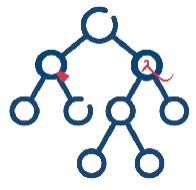
\includegraphics[height=1.0cm]{msca_logo.png}}%
    \end{center}

    \vspace{0.6cm}

    % Main title with Q logos on sides (with clickable links)
    \begin{center}
        \begin{minipage}{0.1\textwidth}
            \centering
            \href{https://quantlet.com}{
\includegraphics[height=1.1cm]{ql_logo.png}}
        \end{minipage}%
        \begin{minipage}{0.78\textwidth}
            \centering
            {\LARGE\bfseries\usebeamercolor[fg]{title}\inserttitle}

            \vspace{0.3cm}

            {\usebeamerfont{subtitle}\usebeamercolor[fg]{title}\insertsubtitle}
        \end{minipage}%
        \begin{minipage}{0.1\textwidth}
            \centering
            \href{https://quantinar.com}{
\includegraphics[height=1.1cm]{qr_logo.png}}
        \end{minipage}
    \end{center}

    \vspace{0.6cm}

    % Authors (left aligned)
    \hspace{0.5cm}{\usebeamerfont{author}\insertauthor}

    \vspace{0.3cm}

    % Institute/Affiliations (left aligned)
    \hspace{0.5cm}\begin{minipage}[t]{0.9\textwidth}
        \raggedright\small\insertinstitute
    \end{minipage}
}

%=============================================================================
% THEOREM ENVIRONMENTS
%=============================================================================
\theoremstyle{definition}
\setbeamertemplate{theorems}[numbered]
\ifdefined\sfmlang
\newtheorem{defn}{Definiție}
\newtheorem{thm}{Teoremă}
\newtheorem{prop}{Propoziție}
\newtheorem{rmk}{Observație}
\else
\newtheorem{defn}{Definition}
\newtheorem{thm}{Theorem}
\newtheorem{prop}{Proposition}
\newtheorem{rmk}{Remark}
\fi

%=============================================================================
% CENTRED MINIPAGE (no extra vertical space)
%=============================================================================
\newenvironment{cminipage}[1]{%
    \par\noindent\hfill\begin{minipage}{#1}\ignorespaces
}{%
    \end{minipage}\hfill\null\par
}

%=============================================================================
% CUSTOM COMMANDS
%=============================================================================
\newcommand{\E}{\mathbb{E}}
\newcommand{\Var}{\text{Var}}
\newcommand{\Cov}{\text{Cov}}
\newcommand{\Corr}{\text{Corr}}
\newcommand{\R}{\mathbb{R}}
\newcommand{\N}{\mathbb{N}}
\newcommand{\Z}{\mathbb{Z}}
\newcommand{\B}{\mathbf{B}}
\newcommand{\imark}{\textcolor{MainBlue}{\textbullet}}
\newcommand{\RMSE}{\text{RMSE}}
\newcommand{\MAE}{\text{MAE}}
\newcommand{\MAPE}{\text{MAPE}}



\newcommand{\qlurl}[1]{https://github.com/danpele/SFM/tree/main/Quantlets/Ch_11/#1}

% Clickable citations (DOIs verified via Crossref)

\newcommand{\refPeters}{\href{https://www.wiley.com/en-us/Fractal+Market+Analysis\%3A+Applying+Chaos+Theory+to+Investment+and+Economics-p-9780471585244}{Peters (1994)}}
\newcommand{\refFama}{\href{https://doi.org/10.2307/2325486}{Fama (1970)}}
\newcommand{\refLoAMH}{\href{https://doi.org/10.3905/jpm.2004.442611}{Lo (2004)}}
\newcommand{\refMan}{\href{https://doi.org/10.1086/294632}{Mandelbrot (1963)}}
\newcommand{\refCoast}{\href{https://doi.org/10.1126/science.156.3775.636}{Mandelbrot (1967)}}
\newcommand{\refMVN}{\href{https://doi.org/10.1137/1010093}{Mandelbrot \& Van Ness (1968)}}
\newcommand{\refNoah}{\href{https://doi.org/10.1029/WR004i005p00909}{Mandelbrot \& Wallis (1968)}}
\newcommand{\refMW}{\href{https://doi.org/10.1029/WR005i005p00967}{Mandelbrot \& Wallis (1969)}}
\newcommand{\refHurst}{\href{https://doi.org/10.1061/TACEAT.0006518}{Hurst (1951)}}
\newcommand{\refAL}{\href{https://doi.org/10.1093/biomet/63.1.111}{Anis \& Lloyd (1976)}}
\newcommand{\refLo}{\href{https://doi.org/10.2307/2938368}{Lo (1991)}}
\newcommand{\refNW}{\href{https://doi.org/10.2307/1913610}{Newey \& West (1987)}}
\newcommand{\refTTW}{\href{https://doi.org/10.1016/S0378-3758(98)00250-X}{Teverovsky, Taqqu \& Willinger (1999)}}
\newcommand{\refPeng}{\href{https://doi.org/10.1103/PhysRevE.49.1685}{Peng et al.\ (1994)}}
\newcommand{\refKan}{\href{https://doi.org/10.1016/S0378-4371(01)00144-3}{Kantelhardt et al.\ (2001)}}
\newcommand{\refGPH}{\href{https://doi.org/10.1111/j.1467-9892.1983.tb00371.x}{Geweke \& Porter-Hudak (1983)}}
\newcommand{\refRob}{\href{https://doi.org/10.1214/aos/1176324317}{Robinson (1995)}}
\newcommand{\refGJ}{\href{https://doi.org/10.1111/j.1467-9892.1980.tb00297.x}{Granger \& Joyeux (1980)}}
\newcommand{\refHosking}{\href{https://doi.org/10.1093/biomet/68.1.165}{Hosking (1981)}}
\newcommand{\refBaillie}{\href{https://doi.org/10.1016/0304-4076(95)01732-1}{Baillie (1996)}}
\newcommand{\refDGE}{\href{https://doi.org/10.1016/0927-5398(93)90006-D}{Ding, Granger \& Engle (1993)}}
\newcommand{\refDI}{\href{https://doi.org/10.1016/S0304-4076(01)00073-2}{Diebold \& Inoue (2001)}}
\newcommand{\refGH}{\href{https://doi.org/10.1016/j.jempfin.2003.03.001}{Granger \& Hyung (2004)}}
\newcommand{\refLS}{\href{https://doi.org/10.1080/07350015.1998.10524760}{Lobato \& Savin (1998)}}
\newcommand{\refCobb}{\href{https://doi.org/10.1093/biomet/65.2.243}{Cobb (1978)}}
\newcommand{\refBBM}{\href{https://doi.org/10.1016/S0304-4076(95)01749-6}{Baillie, Bollerslev \& Mikkelsen (1996)}}
\newcommand{\refAB}{\href{https://doi.org/10.1111/j.1540-6261.1997.tb02722.x}{Andersen \& Bollerslev (1997)}}
\newcommand{\refMuller}{\href{https://doi.org/10.1016/S0927-5398(97)00007-8}{Müller et al.\ (1997)}}
\newcommand{\refCorsi}{\href{https://doi.org/10.1093/jjfinec/nbp001}{Corsi (2009)}}
\newcommand{\refWeron}{\href{https://doi.org/10.1016/S0378-4371(02)00961-5}{Weron (2002)}}
\newcommand{\refCT}{\href{https://doi.org/10.1016/j.physa.2003.12.031}{Cajueiro \& Tabak (2004)}}
\newcommand{\refUrq}{\href{https://doi.org/10.1016/j.econlet.2016.09.019}{Urquhart (2016)}}
\newcommand{\refNC}{\href{https://doi.org/10.1016/j.econlet.2016.10.033}{Nadarajah \& Chu (2017)}}
\newcommand{\refBar}{\href{https://doi.org/10.1016/j.econlet.2017.09.013}{Bariviera (2017)}}
\newcommand{\refKrisA}{\href{https://doi.org/10.1142/S0219525912500658}{Kristoufek (2012)}}
\newcommand{\refKrisB}{\href{https://doi.org/10.1038/srep02857}{Kristoufek (2013)}}
\newcommand{\refCarlson}{\href{https://www.federalreserve.gov/pubs/feds/2007/200713/index.html}{Carlson (2007)}}
\newcommand{\refRogers}{\href{https://doi.org/10.1111/1467-9965.00025}{Rogers (1997)}}
\newcommand{\refFHH}{\href{https://doi.org/10.1007/978-3-030-13751-9}{Franke, Härdle \& Hafner (2019)}}
\newcommand{\refWang}{\href{https://doi.org/10.1038/s41586-023-06221-2}{Wang et al.\ (2023)}}
\newcommand{\refPeleA}{\href{https://doi.org/10.1016/j.sbspro.2012.09.1030}{Pele \& Mazurencu-Marinescu (2012)}}
\newcommand{\refPeleB}{\href{https://doi.org/10.5018/economics-ejournal.ja.2019-29}{Pele \& Mazurencu-Marinescu-Pele (2019)}}

\title[Statistics of Financial Markets]{Statistics of Financial Markets}
\subtitle{Chapter 11: Fractal markets hypothesis and long memory}
\author[D.T. Pele]{Daniel Traian PELE}
\institute{Bucharest University of Economic Studies\\
IDA Institute Digital Assets\\
Blockchain Research Center\\
AI4EFin Artificial Intelligence for Energy Finance\\
Romanian Academy, Institute for Economic Forecasting\\
MSCA Digital Finance}
\date{}

%=============================================================================
\providecommand{\sfmapplink}[3]{\hypertarget{#2}{}\hyperlink{#1}{\beamergotobutton{#3}}}  % APPLINKS-MACROS
\providecommand{\sfmappback}[2]{\begin{tikzpicture}[remember picture,overlay]\node[anchor=south east] at ([xshift=-3mm,yshift=7mm]current page.south east){\hyperlink{#1}{\beamerreturnbutton{#2}}};\end{tikzpicture}}  % APPLINKS-MACROS
\providecommand{\sfmchlink}[2]{\href{#1}{#2}}  % APPLINKS-MACROS
\providecommand{\sfmchlinkt}[2]{\href{#1}{\usebeamercolor[fg]{frametitle}#2}}  % APPLINKS-MACROS
\begin{document}
%=============================================================================

{
\setbeamertemplate{headline}{}
\setbeamertemplate{footline}{}
\begin{frame}[noframenumbering]
    \titlepage
\end{frame}
}
% BEGIN-ACRONYMS (generat de latex/acronyms.py; nu editati manual)
\begin{frame}{Acronyms used in this material}
\setbeamertemplate{itemize/enumerate body begin}{\footnotesize}
\begin{columns}[T]
\begin{column}{0.49\textwidth}
\begin{itemize}\setlength{\itemsep}{0pt}
    \item \textbf{ACF}: Autocorrelation Function
    \item \textbf{AI}: Artificial Intelligence
    \item \textbf{AMH}: Adaptive Markets Hypothesis
    \item \textbf{AR}: AutoRegressive (model); Abnormal Return
    \item \textbf{ARFIMA}: AutoRegressive Fractionally Integrated Moving Average
    \item \textbf{ARMA}: AutoRegressive Moving Average (model)
    \item \textbf{BET}: Bucharest Exchange Trading (index)
    \item \textbf{BET-TR}: BET Total Return (index)
    \item \textbf{BVB}: Bursa de Valori București (the Bucharest Stock Exchange)
    \item \textbf{DFA}: Detrended Fluctuation Analysis
    \item \textbf{EMH}: Efficient Market Hypothesis
\end{itemize}
\end{column}
\begin{column}{0.49\textwidth}
\begin{itemize}\setlength{\itemsep}{0pt}
    \item \textbf{EODHD}: EOD Historical Data (market-data provider)
    \item \textbf{FIGARCH}: Fractionally Integrated GARCH
    \item \textbf{FMH}: Fractal Market Hypothesis
    \item \textbf{GARCH}: Generalised AutoRegressive Conditional Heteroskedasticity
    \item \textbf{GPH}: Geweke–Porter-Hudak (log-periodogram estimator)
    \item \textbf{HAR}: Heterogeneous AutoRegressive (model)
    \item \textbf{IGARCH}: Integrated GARCH
    \item \textbf{MA}: Moving Average
    \item \textbf{OLS}: Ordinary Least Squares
    \item \textbf{SE}: Standard Error
    \item \textbf{SFE}: Statistics of Financial Markets, Exercises (Quantlet collection of the textbook)
    \item \textbf{US}: United States
\end{itemize}
\end{column}
\end{columns}
\end{frame}
% END-ACRONYMS

\begin{frame}{Today's Question and Route}
\itemsize{\small}
\begin{itemize}
    \item \textbf{Question}: do today's returns remember what happened months ago?
    \begin{itemize}
        \item the fractal market hypothesis adds a second theme: who trades, and at which horizon
        \item \sfmchlink{https://danpele.github.io/SFM/EN/Courses/chapter7_efficient_markets_random_walk_vr.pdf}{Chapter 7}: daily returns are almost uncorrelated at short lags; \sfmchlink{https://danpele.github.io/SFM/EN/Courses/chapter8_volatility_estimators.pdf}{Chapters 8} and \sfmchlink{https://danpele.github.io/SFM/EN/Courses/chapter9_arch_garch_models.pdf}{9}: volatility is persistent
        \item this chapter asks about dependence over \textbf{long} lags and over \textbf{many} time scales
    \end{itemize}
    \item \textbf{Route} of the chapter
    \begin{itemize}
        \item the fractal market hypothesis of Peters; self-similarity and fractals
        \item Hurst and the Nile; the R/S statistic; long memory, fractional Brownian motion, ARFIMA
        \item estimators (R/S, Lo, DFA, GPH), Monte Carlo bands, spurious long memory
        \item long memory in volatility; rolling Hurst exponents on six markets; consequences for risk
    \end{itemize}
\end{itemize}
\end{frame}

\begin{frame}{Learning Outcomes}
\itemsize{\small}
\begin{itemize}
    \item State the fractal market hypothesis and compare it with the efficient and the adaptive market hypotheses
    \item Define self-similarity, the Hurst exponent, fractional Brownian motion, fractional Gaussian noise and ARFIMA(0,$d$,0)
    \item Compute the R/S statistic step by step and estimate $H$ with R/S, DFA and the GPH regression; apply Lo's modified R/S test
    \item Judge an estimate against Monte Carlo bands and recognise spurious long memory (breaks, volatility clustering)
    \item Separate long memory in returns from long memory in volatility on real data, with rolling estimates
    \item Explain how $H$ changes the scaling of risk with the horizon
\end{itemize}
\end{frame}

\begin{frame}{Reading and Tools}
\itemsize{\small}
\begin{itemize}
    \item Textbook: \refFHH, Ch.~14 (14.1--14.5 definition, fractional integration, self-similarity, tests and estimators of long memory; 14.6 long memory models)
    \begin{itemize}
        \item the fractal market hypothesis: \refPeters; a survey of long memory: \refBaillie
    \end{itemize}
    \item Python Quantlets of this chapter: \href{https://github.com/danpele/SFM/tree/main/Quantlets/Ch_11}{Quantlets/Ch\_11}
    \begin{itemize}
        \item ported from the SFE Quantlets SFEfbmplot, SFEfgnacf and SFEarfima
    \end{itemize}
    \item Lecture notebook: \href{\colaburl{notebooks/EN/chapter11_lecture_notebook.ipynb}}{open in Google Colab}
    \item Video courses: \quantinar{Efficiency of cryptocurrency markets}{https://quantinar.com/course/184/efficiency-of-cryptocurrency-markets-a-gmm-based-analysis}; \quantinar{Applied Time Series Analysis with Python}{https://quantinar.com/course/137/applied-time-series-analysis-with-python}
    \item Further reading on crashes and power laws in Romanian and crypto markets: \refPeleA; \refPeleB
\end{itemize}
\end{frame}


%=============================================================================
\section{From Efficient to Fractal Markets}
%=============================================================================

\begin{frame}{What the EMH Leaves Open}
\itemsize{\small}
\begin{itemize}
    \item EMH (efficient market hypothesis, \refFama; \sfmchlink{https://danpele.github.io/SFM/EN/Courses/chapter7_efficient_markets_random_walk_vr.pdf}{Chapter 7}): prices reflect the available information, so returns cannot be forecast from past returns
    \begin{itemize}
        \item the random walk of prices implies independent increments: in this chapter, $H = 0.5$
    \end{itemize}
    \item Facts that the random walk with Normal increments does not explain
    \begin{itemize}
        \item heavy tails (\sfmchlink{https://danpele.github.io/SFM/EN/Courses/chapter2_classical_distributions_stylised_facts.pdf}{Chapters 2}, \sfmchlink{https://danpele.github.io/SFM/EN/Courses/chapter3_alpha_stable_distributions.pdf}{3}, \sfmchlink{https://danpele.github.io/SFM/EN/Courses/chapter5_heavy_tails_evt.pdf}{5}); volatility clustering (\sfmchlink{https://danpele.github.io/SFM/EN/Courses/chapter8_volatility_estimators.pdf}{Chapters 8}, \sfmchlink{https://danpele.github.io/SFM/EN/Courses/chapter9_arch_garch_models.pdf}{9})
        \item crashes such as that of 19 October 1987 (a few slides ahead)
    \end{itemize}
    \item The EMH says nothing about \textbf{who} trades and at which \textbf{horizon}: all investors are treated as one representative investor
\end{itemize}
\end{frame}

\begin{frame}{Edgar Peters and the Fractal Market Hypothesis}
\itemsize{\footnotesize}
\begin{itemize}
    \item \textbf{FMH} (fractal market hypothesis) \refPeters: the market is made of investors with \textbf{many investment horizons}, from minutes to decades
    \item The five statements of Peters
    \begin{itemize}
        \item the market is stable when it contains investors with many different horizons: this ensures liquidity
        \item short horizons react to sentiment and technical information; long horizons react to fundamental information
        \item if the fundamental information becomes doubtful, long-term investors leave or start to trade short term: horizons become uniform and the market becomes unstable
        \item prices combine short-term technical trading and long-term fundamental valuation
        \item an asset without a link to the economic cycle has no long-term trend: short-term trading and liquidity dominate
    \end{itemize}
\end{itemize}
\end{frame}

\begin{frame}{Investment Horizons and Liquidity: an Example}
\itemsize{\small}
\begin{itemize}
    \item A share falls by 3\% in one morning
    \begin{itemize}
        \item a day trader (horizon: hours) sees a large move and sells
        \item a pension fund (horizon: ten years) sees a small move relative to its horizon and buys at a lower price
    \end{itemize}
    \item The long-horizon investor supplies the liquidity that the short-horizon investor demands: the price stays orderly
    \item If the pension fund also starts to fear the next hours, nobody buys: there is no liquidity and the fall accelerates
    \item \textbf{Fractal}: the same pattern of behaviour repeats at every horizon, with statistically similar returns at different scales
\end{itemize}
\end{frame}

\begin{frame}{1987: a Crash as a Collapse of Horizons}
\itemsize{\footnotesize}
\begin{columns}[T]
\begin{column}{0.52\textwidth}
\begin{itemize}
    \item 19 October 1987: the S\&P 500 fell by about 20\% in one day \refCarlson
    \item The FMH reading
    \begin{itemize}
        \item portfolio insurance and program trading made long-term portfolios sell like short-term traders
        \item all horizons became one horizon: buyers disappeared
    \end{itemize}
    \item Testable consequence: in crises, short horizons dominate and the statistical structure across scales changes
\end{itemize}
\end{column}
\begin{column}{0.44\textwidth}
\centering
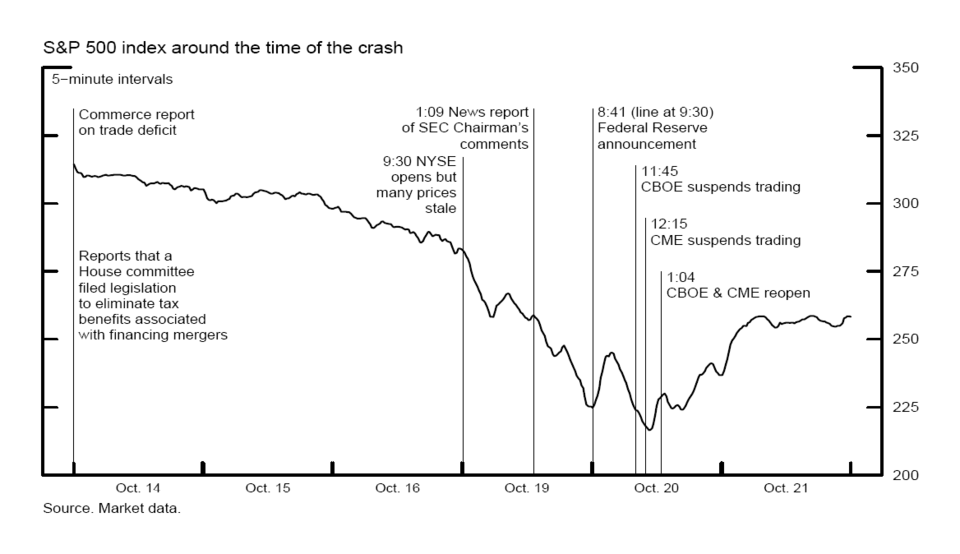
\includegraphics[height=0.36\textheight]{ch11_sp500_1987_fed.png}\\[1mm]
\imgcap{The S\&P 500 around the crash of October 1987}
\imgcredit{https://commons.wikimedia.org/wiki/File:S\%26P_500_index_around_the_time_of_the_crash.png}{Chart: Mark Carlson, Federal Reserve Board (2006); public domain; Wikimedia Commons}
\end{column}
\end{columns}
\end{frame}

\begin{frame}{Testing the FMH: Scaling, Horizons and Liquidity}
\itemsize{\small}
\begin{itemize}
    \item The FMH is a verbal theory; its statistical consequences can be tested
    \begin{itemize}
        \item \textbf{self-similarity}: the distribution of $h$-day returns looks the same after rescaling by $h^H$ (Section 2)
        \item \textbf{memory}: the Hurst exponent $H$ measures dependence over long horizons (Sections 3--5)
        \item \textbf{change}: in crises, $H$ and the share of short horizons should change (Section 8)
    \end{itemize}
    \item Landmark evidence: \refKrisA\ and \refKrisB\ on the 2008 crisis
    \begin{itemize}
        \item local Hurst exponents and wavelet power of US and European indices
        \item the most turbulent periods coincide with a dominance of short investment horizons, as the FMH predicts
    \end{itemize}
\end{itemize}
\end{frame}

\begin{frame}{EMH, FMH and AMH}
\itemsize{\small}
\begin{center}
\footnotesize
\begin{tabular}{>{\raggedright\arraybackslash}p{2.2cm}>{\raggedright\arraybackslash}p{2.9cm}>{\raggedright\arraybackslash}p{2.9cm}>{\raggedright\arraybackslash}p{2.9cm}}
\toprule
 & \textbf{EMH} & \textbf{FMH} & \textbf{AMH} \\
\midrule
Source & \refFama{} & \refPeters{} & \refLoAMH{} \\
Investors & one representative investor & many horizons & species that compete and adapt \\
Stability & prices always fair & diversity of horizons gives liquidity & changes with the environment \\
Memory & $H = 0.5$ & $H$ may differ from 0.5 & $H$ varies over time \\
Crises & outside the theory & collapse of horizons & mass extinction of strategies \\
\bottomrule
\end{tabular}
\end{center}
\begin{itemize}
    \item The three are not rival tests: the FMH and the AMH explain when and why the EMH approximation fails
\end{itemize}
\end{frame}


%=============================================================================
\section{Self-Similarity and Fractals}
%=============================================================================

\begin{frame}{Benoît Mandelbrot: Roughness as a Measure}
\itemsize{\footnotesize}
\begin{columns}[T]
\begin{column}{0.58\textwidth}
\begin{itemize}
    \item \refMan: cotton prices have heavy tails and look alike at daily, monthly and yearly scales
    \begin{itemize}
        \item the $\alpha$-stable distributions of \sfmchlink{https://danpele.github.io/SFM/EN/Courses/chapter3_alpha_stable_distributions.pdf}{Chapter 3}
    \end{itemize}
    \item \refCoast: the measured length of a coast grows as the ruler shrinks; the growth rate defines a \textbf{fractal dimension}
    \item \refMVN: fractional Brownian motion, the model of this chapter
    \item \textbf{Fractal}: an object whose parts resemble the whole, exactly or in distribution
\end{itemize}
\end{column}
\begin{column}{0.38\textwidth}
\centering
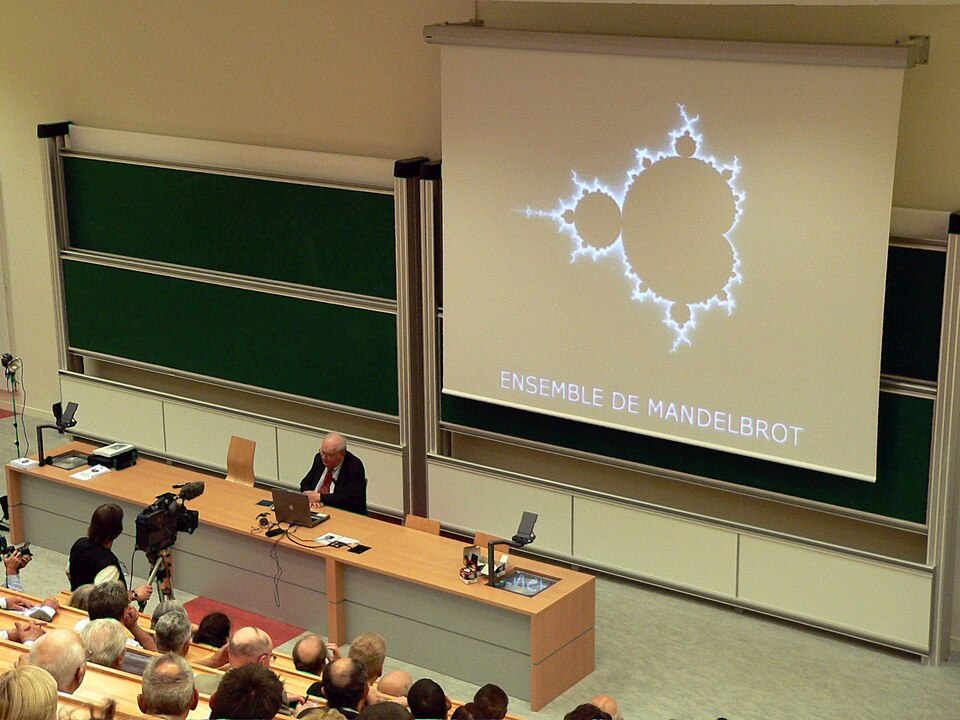
\includegraphics[height=0.25\textheight]{ch11_mandelbrot_2006.jpg}\\[1mm]
\imgcap{Benoît Mandelbrot (1924--2010), Paris, 2006}
\imgcredit{https://commons.wikimedia.org/wiki/File:Mandelbrot_p1130876.jpg}{Photo: David Monniaux (2006); CC BY-SA 3.0; Wikimedia Commons}\\[1mm]
\centering

\includegraphics[height=0.15\textheight]{ch11_mandelbrot_set.jpg}\\[1mm]
\imgcap{The Mandelbrot set}
\imgcredit{https://commons.wikimedia.org/wiki/File:Mandel_zoom_00_mandelbrot_set.jpg}{Image: Wolfgang Beyer; CC BY-SA 3.0; Wikimedia Commons}
\end{column}
\end{columns}
\end{frame}

\begin{frame}{Fractal Dimension}
\itemsize{\small}
\begin{itemize}
    \item \textbf{Similarity dimension}: an object made of $N$ copies of itself, each scaled by $1/s$, has $D = \ln N/\ln s$
    \begin{itemize}
        \item a segment: 2 halves, $D = \ln 2/\ln 2 = 1$; a square: 4 quarters of side $1/2$, $D = \ln 4/\ln 2 = 2$
        \item the Koch curve: 4 copies scaled by $1/3$, $D = \ln 4/\ln 3 = 1.262$
        \item the Sierpinski triangle: 3 copies scaled by $1/2$, $D = \ln 3/\ln 2 = 1.585$
    \end{itemize}
    \item The west coast of Britain: $D \approx 1.25$ \refCoast
    \item The graph of a price path: $D = 2 - H$
    \begin{itemize}
        \item Brownian motion: $D = 1.5$; a smoother, trending path ($H > 0.5$) has $D < 1.5$
    \end{itemize}
\end{itemize}
\end{frame}

\begin{frame}{Self-Similar Processes}
\itemsize{\small}
\begin{itemize}
    \item \textbf{Self-similar process} \refFHH, Def.~14.1: $X_{ct} \overset{d}{=} c^H X_t$ for every $c > 0$; $H$ is the \textbf{Hurst exponent}
    \begin{itemize}
        \item $\overset{d}{=}$: equal in distribution; stretching time by $c$ equals stretching values by $c^H$
    \end{itemize}
    \item Brownian motion (\sfmchlink{https://danpele.github.io/SFM/EN/Courses/chapter4_probability.pdf}{Chapter 4}) is self-similar with $H = 1/2$: $W_{ct} \overset{d}{=} \sqrt{c}\,W_t$
    \item Consequence for log prices with self-similar increments
    \begin{itemize}
        \item $\mathrm{sd}(r_t^{(h)}) = h^H\,\mathrm{sd}(r_t)$, where $r_t^{(h)}$ is the $h$-day return and sd the standard deviation
        \item the square-root-of-time rule $\sqrt{h}$ is the special case $H = 1/2$
    \end{itemize}
    \item A first estimator of $H$: the slope of $\ln \mathrm{sd}(r^{(h)})$ on $\ln h$
\end{itemize}
\end{frame}

\begin{frame}{The Scaling of $h$-Day Returns}
\itemsize{\footnotesize}
\begin{center}
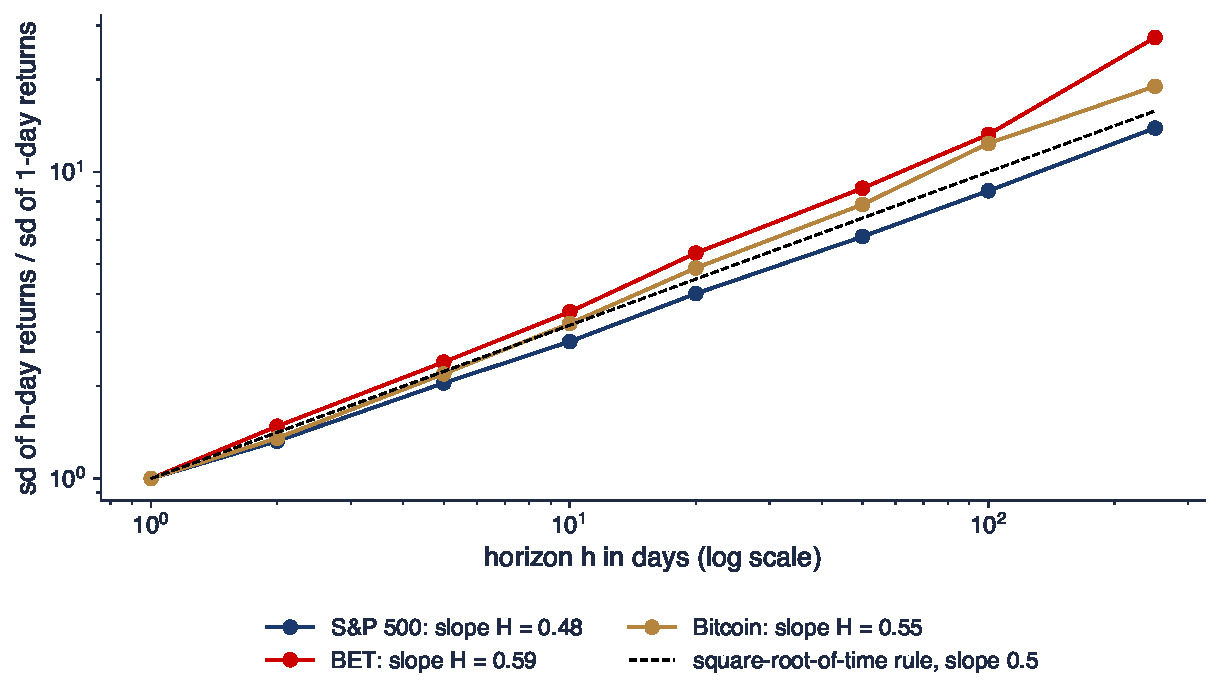
\includegraphics[width=0.97\textwidth,height=0.50\textheight,keepaspectratio]{sfm_ch11_scaling.pdf}
\end{center}
\vspace{-0.25cm}
\begin{itemize}
    \item Standard deviation of non-overlapping $h$-day returns divided by the daily one, $h = 1, \dots, 250$, log scales; data to 18 September 2026
    \item Slopes: S\&P 500 $0.48$, BET $0.59$, Bitcoin $0.55$; the square-root rule has slope 0.5
\end{itemize}
\sfmquantlet{Ch_11}{SFM_ch11_self_similarity}
\end{frame}

\begin{frame}{Interpretation: Scaling Exponents}
\itemsize{\small}
\begin{itemize}
    \item S\&P 500: 10-day risk is $2.80$ times the daily risk, below $\sqrt{10} = 3.16$
    \begin{itemize}
        \item slight mean reversion: daily returns have a negative first-order autocorrelation, $-0.099$
    \end{itemize}
    \item BET: $3.50$ times, above $\sqrt{10}$: positive autocorrelation
    \begin{itemize}
        \item thin trading in the early years makes the index adjust slowly (\sfmchlink{https://danpele.github.io/SFM/EN/Courses/chapter7_efficient_markets_random_walk_vr.pdf}{Chapter 7})
    \end{itemize}
    \item Bitcoin: $3.20$ times, close to $\sqrt{10}$
    \item Caution: there are only a few dozen non-overlapping 250-day blocks; the slope is imprecise, so it needs a proper estimator and a band
\end{itemize}
\end{frame}


%=============================================================================
\section{Hurst, the Nile and the R/S Statistic}
%=============================================================================

\begin{frame}{Harold Edwin Hurst and the Nile}
\itemsize{\footnotesize}
\begin{columns}[T]
\begin{column}{0.60\textwidth}
\begin{itemize}
    \item Hurst (1880--1978), a British hydrologist who worked in Egypt from 1906, designed reservoirs on the Nile
    \begin{itemize}
        \item the capacity needed to deliver the average flow every year equals the range of the cumulative deviations of the inflows from their mean
    \end{itemize}
    \item \refHurst: for independent inflows this range grows like $n^{0.5}$; in river flows, rainfall and tree rings it grows like $n^{K}$ with $K$ about $0.73$ on average
    \begin{itemize}
        \item years of high flow follow years of high flow: \textbf{long memory}
    \end{itemize}
\end{itemize}
\end{column}
\begin{column}{0.36\textwidth}
\centering
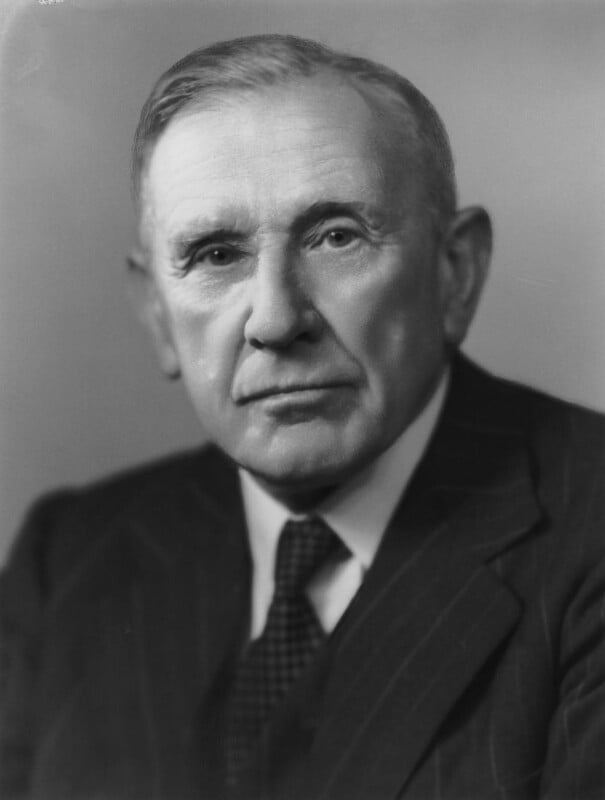
\includegraphics[height=0.24\textheight]{ch11_hurst_1953.jpg}\\[1mm]
\imgcap{H.E. Hurst (1953)}
\imgcredit{https://commons.wikimedia.org/wiki/File:Harold_Edwin_Hurst_in_1953.jpg}{Photo: Elliott \& Fry (1953); public domain; Wikimedia Commons}\\[1mm]
\centering
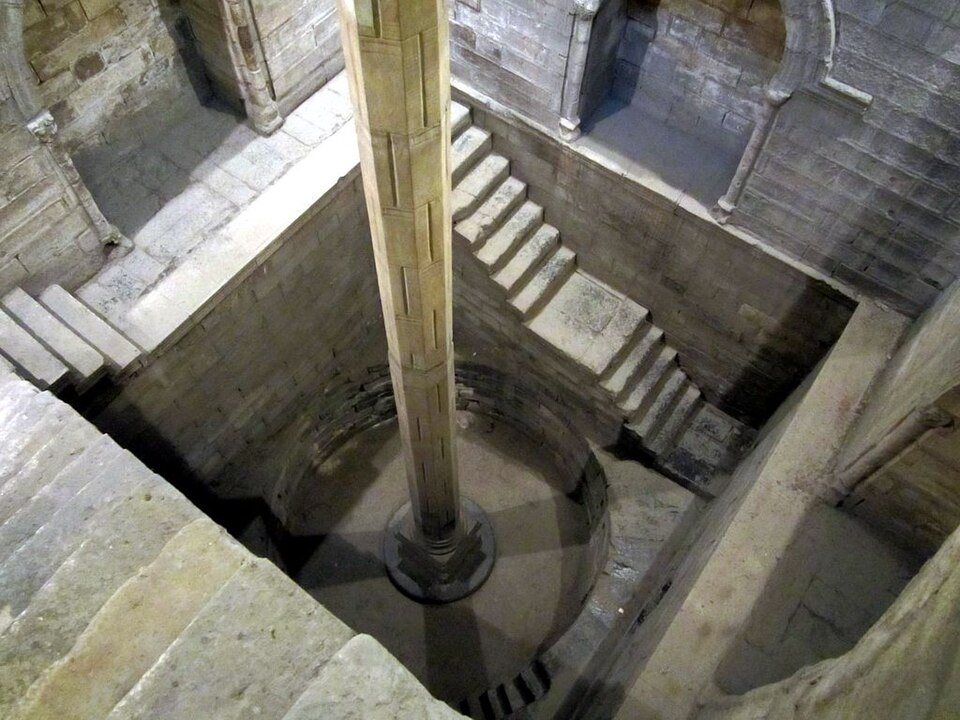
\includegraphics[height=0.17\textheight]{ch11_nilometer_roda.jpg}\\[1mm]
\imgcap{The Nilometer on Roda Island, Cairo, built in 861}
\imgcredit{https://commons.wikimedia.org/wiki/File:Nilometer_(8590204613).jpg}{Photo: David Stanley (2013); CC BY 2.0; Wikimedia Commons}
\end{column}
\end{columns}
\end{frame}

\begin{frame}{The R/S Statistic}
\itemsize{\small}
\begin{itemize}
    \item Block $x_1, \dots, x_n$ with mean $\bar x$; \textbf{cumulative deviations} $Y_k = \sum_{j=1}^{k}(x_j - \bar x)$, $k = 1, \dots, n$
    \begin{itemize}
        \item $Y_n = 0$ by construction
    \end{itemize}
    \item \textbf{Range}: $R_n = \max_k Y_k - \min_k Y_k$; \textbf{standard deviation}: $S_n = \sqrt{\tfrac1n\sum_j (x_j - \bar x)^2}$
    \item \textbf{R/S statistic} (rescaled range) \refFHH, 14.4.1: $(R/S)_n = R_n/S_n$
    \begin{itemize}
        \item dividing by $S_n$ removes the unit: $(R/S)_n$ is comparable across assets
        \item for i.i.d.\ data with finite variance, $(R/S)_n$ grows like $n^{1/2}$; under long memory like $n^H$, $H > 1/2$
    \end{itemize}
    \item Robust to heavy tails: $R$ and $S$ are inflated by the same extreme values \refMW
\end{itemize}
\end{frame}

\begin{frame}{Worked Example: R/S of Eight Returns}
\itemsize{\scriptsize}
\begin{columns}[T]
\begin{column}{0.52\textwidth}
\begin{itemize}
    \item Returns (\%): $0.5;\ -0.3;\ 0.8;\ -0.2;\ 0.6;\ -0.1;\ 0.4;\ -0.7$
    \item Mean $\bar x = 1.0/8 = 0.125$
    \item Deviations: $+0.375$, $-0.425$, $+0.675$, $-0.325$, $+0.475$, $-0.225$, $+0.275$, $-0.825$
    \item $Y_k$: $0.375$, $-0.050$, $0.625$, $0.300$, $0.775$, $0.550$, $0.825$, $0.000$
    \item $R = 0.825 - (-0.050) = 0.875$; $S = \sqrt{1.915/8} = 0.489$
    \item $(R/S)_8 = 0.875/0.489 = 1.788$; one block gives one point, $H$ needs many block sizes
\end{itemize}
\end{column}
\begin{column}{0.46\textwidth}
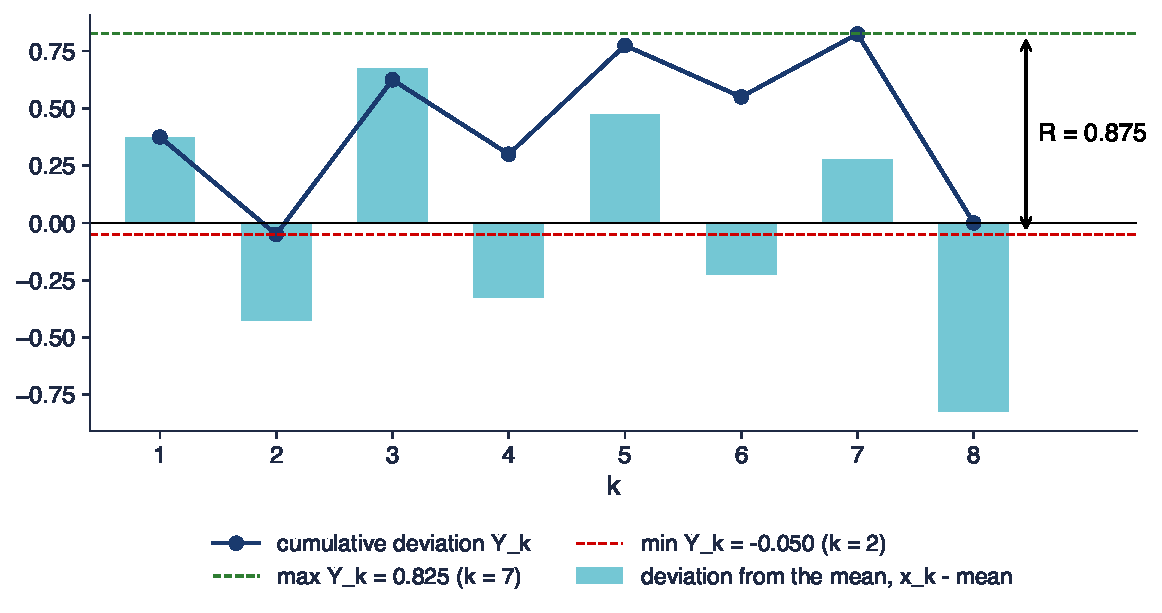
\includegraphics[width=\textwidth]{sfm_ch11_rs_example.pdf}
\sfmquantlet{Ch_11}{SFM_ch11_rs_estimators}
\end{column}
\end{columns}
\end{frame}

\begin{frame}{From R/S to the Hurst Exponent}
\itemsize{\small}
\begin{itemize}
    \item Steps \refMW
    \begin{itemize}
        \item choose block sizes $n$ between 10 and $N/4$, evenly spaced on a log scale
        \item split the $N$ returns into $\lfloor N/n\rfloor$ non-overlapping blocks; compute $R/S$ in each block and average: $(R/S)_n$
        \item regress $\ln (R/S)_n = \ln c + H \ln n + e_n$ by OLS (ordinary least squares): the slope $\hat H$ estimates $H$
        \item $N$: the number of returns; $n$: the block size; $c$: a constant; $e_n$: the regression error
    \end{itemize}
    \item The log-log plot is the main diagnostic: a straight line supports a single scaling exponent
    \item Applied to returns (stationary), not to prices: for prices, $(R/S)_n$ grows like $n$
\end{itemize}
\end{frame}

\begin{frame}{Interpreting $H$}
\itemsize{\small}
\begin{center}
\footnotesize
\begin{tabular}{llll}
\toprule
$H$ & increments & memory & path ($D = 2 - H$) \\
\midrule
$0 < H < 0.5$ & negatively correlated & anti-persistent: reversals & rough, $D > 1.5$ \\
$H = 0.5$ & uncorrelated & none (random walk) & $D = 1.5$ \\
$0.5 < H < 1$ & positively correlated & persistent: trends & smoother, $D < 1.5$ \\
\bottomrule
\end{tabular}
\end{center}
\begin{itemize}
    \item $H$ is not a probability: $H = 0.7$ does not mean ``70\% chance that the sign repeats''
    \item Two effects named by \refNoah
    \begin{itemize}
        \item \textbf{Noah effect}: extreme values (heavy tails, the flood); \textbf{Joseph effect}: long runs of high or low values (``seven years of plenty, seven years of famine'')
        \item $H$ measures the Joseph effect; the tail index of \sfmchlink{https://danpele.github.io/SFM/EN/Courses/chapter5_heavy_tails_evt.pdf}{Chapter 5} measures the Noah effect
    \end{itemize}
\end{itemize}
\end{frame}

\begin{frame}{Small Samples: the Bias of R/S}
\itemsize{\small}
\begin{itemize}
    \item For i.i.d.\ data, $(R/S)_n$ approaches $c\,n^{1/2}$ only for large $n$; for small $n$ it grows faster \refAL
    \begin{itemize}
        \item the fitted slope over $n = 10, \dots, N/4$ is above 0.5 even without any memory
    \end{itemize}
    \item Monte Carlo, 500 i.i.d.\ Normal series
    \begin{itemize}
        \item mean $\hat H_{R/S}$: $0.588$ for $N = 250$, $0.562$ for $N = 1000$, $0.547$ for $N = 5000$
        \item 95\% band for $N = 1000$: $[0.50, 0.63]$
    \end{itemize}
    \item Rule: compare $\hat H$ with the distribution of $\hat H$ under the null hypothesis for the same $N$, not with 0.5 (Section 5)
\end{itemize}
\end{frame}


%=============================================================================
\section{Long Memory: Definitions and Models}
%=============================================================================

\begin{frame}{Short and Long Memory}
\itemsize{\small}
\begin{itemize}
    \item Stationary $X_t$ with autocorrelations $\rho(k)$ (ACF, autocorrelation function); \textbf{long memory} \refFHH, 14.1:
    \begin{itemize}
        \item $\sum_{k} |\rho(k)| = \infty$: the autocorrelations are not summable
        \item equivalently, hyperbolic decay $\rho(k) \sim C\,k^{2d - 1}$ as $k \to \infty$, with the \textbf{memory parameter} $0 < d < 0.5$
        \item in frequency: the spectral density has a pole at zero, $f(\lambda) \sim C\,\lambda^{-2d}$ as $\lambda \to 0$
        \item $C > 0$: a constant; $\sim$: the ratio of the two sides tends to 1; $f(\lambda)$: the share of variance at frequency $\lambda$ (long cycles: $\lambda$ near 0)
    \end{itemize}
    \item \textbf{Short memory}: ARMA (autoregressive moving average) models, e.g.\ AR(1) with $\rho(k) = \phi^k$
    \begin{itemize}
        \item exponential decay: $\sum_k |\phi|^k = 1/(1 - |\phi|) < \infty$
    \end{itemize}
    \item Link with the Hurst exponent: $d = H - 1/2$
\end{itemize}
\end{frame}

\begin{frame}{Worked Example: How Fast Does Memory Fade?}
\itemsize{\small}
\begin{itemize}
    \item Long memory: fractional Gaussian noise (next slides) with $H = 0.8$
    \begin{itemize}
        \item $\rho(1) = 2^{2H - 1} - 1 = 2^{0.6} - 1 = 0.516$
        \item $\rho(10) = 0.191$, $\rho(50) = 0.100$, $\rho(100) = 0.076$
    \end{itemize}
    \item Short memory: AR(1) with the same first autocorrelation, $\phi = 0.516$
    \begin{itemize}
        \item $\rho(10) = \phi^{10} = 0.0013$; $\rho(100) = \phi^{100}$, practically zero
    \end{itemize}
    \item Same short-run behaviour, very different long run: after 100 days, a shock still matters only under long memory
\end{itemize}
\end{frame}

\begin{frame}{Fractional Brownian Motion}
\itemsize{\small}
\begin{itemize}
    \item \textbf{Fractional Brownian motion} (fBm) $B_H(t)$, $0 < H < 1$ \refMVN; \refFHH, Def.~14.2: a Gaussian process with continuous paths, self-similar with exponent $H$ and with stationary increments
    \item Properties (\refFHH, Th.~14.1)
    \begin{itemize}
        \item $B_H(0) = 0$, $E[B_H(t)] = 0$, $E[B_H(t)^2] = \sigma^2 |t|^{2H}$ ($\sigma^2$: the variance at $t = 1$)
        \item $\mathrm{Cov}(B_H(t), B_H(s)) = \tfrac{\sigma^2}{2}\left(|t|^{2H} + |s|^{2H} - |t - s|^{2H}\right)$
    \end{itemize}
    \item $H = 1/2$: Brownian motion, independent increments; $H \neq 1/2$: the increments are correlated at all lags
    \item Simulation: exact, from the covariance matrix of the increments (circulant embedding, as in the notebook)
\end{itemize}
\end{frame}

\begin{frame}{fBm Paths for Three Hurst Exponents}
\itemsize{\footnotesize}
\begin{center}
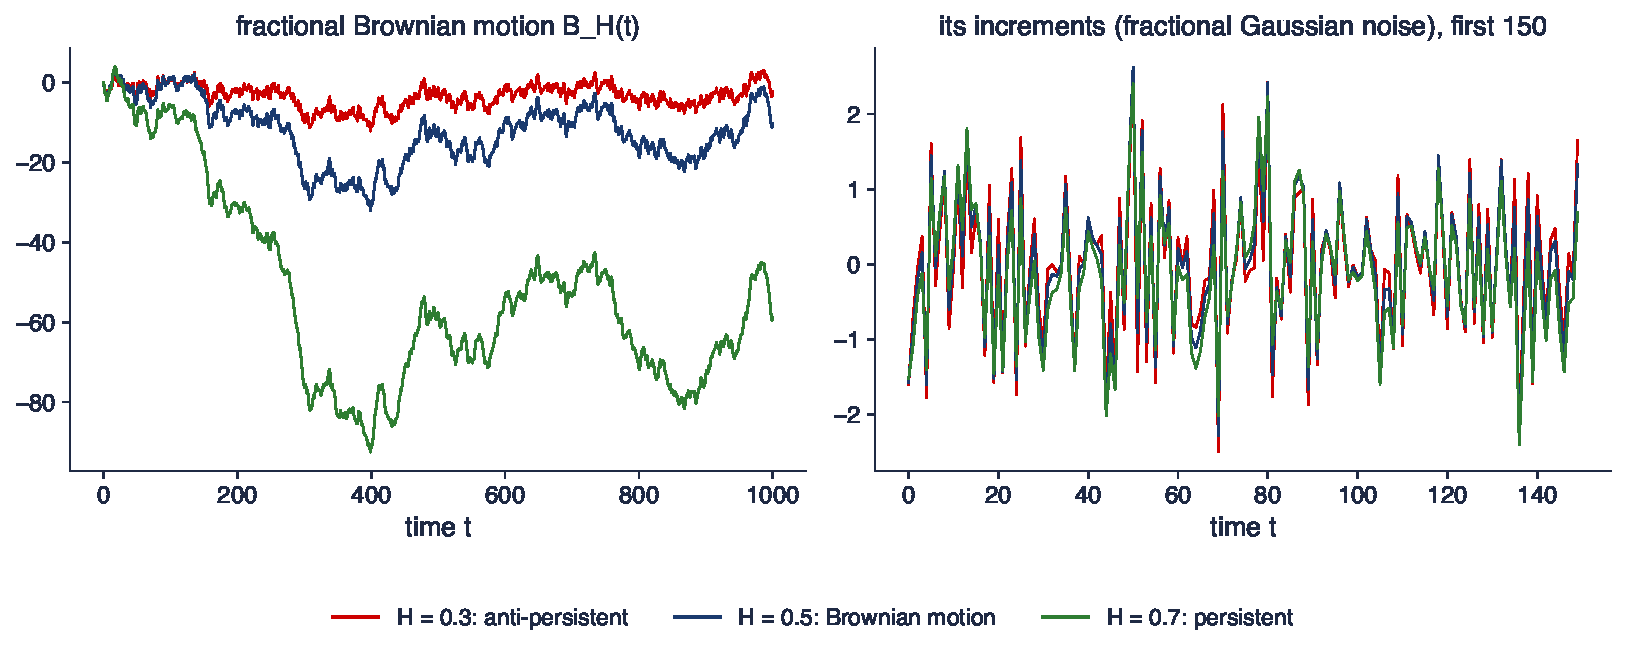
\includegraphics[width=0.97\textwidth,height=0.52\textheight,keepaspectratio]{sfm_ch11_fbm_paths.pdf}
\end{center}
\vspace{-0.25cm}
\begin{itemize}
    \item The same random numbers, $H = 0.3$, $0.5$, $0.7$ (as in SFEfbmplot); right: the first 150 increments
    \item $H = 0.7$: long excursions and a wide range; $H = 0.3$: frequent reversals, a narrow range; lag-1 autocorrelation of the increments $0.32$ and $-0.23$ (theory $0.32$ and $-0.24$)
\end{itemize}
\sfmquantlet{Ch_11}{SFM_ch11_fbm_fgn}
\end{frame}

\begin{frame}{Fractional Gaussian Noise}
\itemsize{\small}
\begin{itemize}
    \item \textbf{Fractional Gaussian noise} (fGn): the increments $Y_k = B_H(k + 1) - B_H(k)$, a stationary series \refFHH, 14.3
    \begin{itemize}
        \item $\rho(k) = \tfrac12\left(|k + 1|^{2H} - 2|k|^{2H} + |k - 1|^{2H}\right)$
        \item for large $k$: $\rho(k) \approx H(2H - 1)\,k^{2H - 2}$
    \end{itemize}
    \item Three regimes
    \begin{itemize}
        \item $1/2 < H < 1$: $\rho(k) > 0$ and not summable: long memory with $d = H - 1/2 \in (0, 1/2)$
        \item $H = 1/2$: white noise
        \item $0 < H < 1/2$: $\rho(k) < 0$, summable: anti-persistence
    \end{itemize}
    \item fGn is the model behind R/S and DFA: for fGn data, both estimate $H$
\end{itemize}
\end{frame}

\begin{frame}{The ACF of Fractional Gaussian Noise}
\itemsize{\footnotesize}
\begin{center}
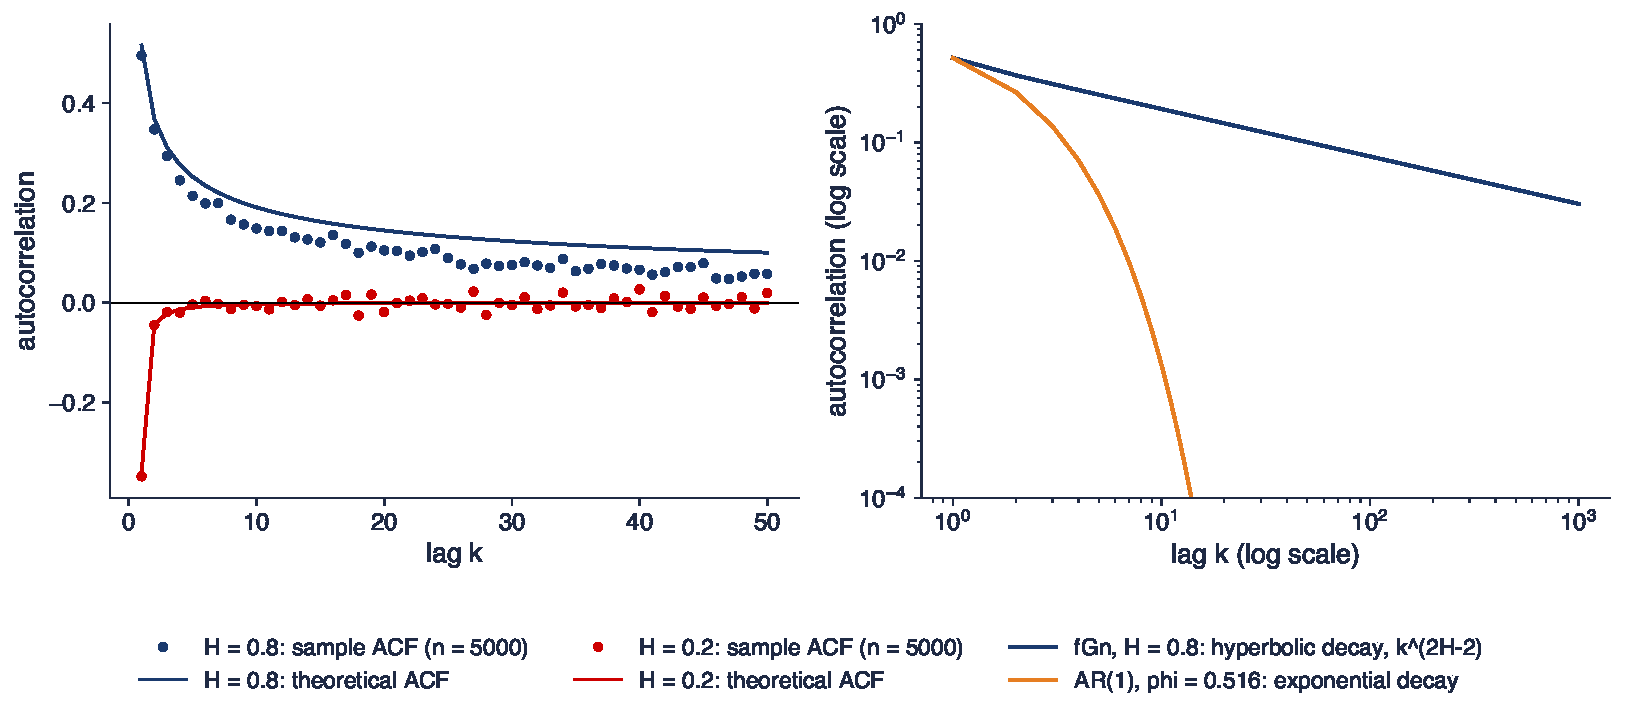
\includegraphics[width=0.97\textwidth,height=0.48\textheight,keepaspectratio]{sfm_ch11_fgn_acf.pdf}
\end{center}
\vspace{-0.25cm}
\begin{itemize}
    \item Left: sample and theoretical ACF for $H = 0.8$ and $H = 0.2$ (as in SFEfgnacf); $\rho(1) = 0.516$ and $-0.340$
    \item Right, log scales: hyperbolic decay (a straight line) against the exponential decay of an AR(1) with the same $\rho(1)$
    \item The sample ACF of a long-memory series lies below the theoretical one: estimating the mean removes part of the slow component
\end{itemize}
\sfmquantlet{Ch_11}{SFM_ch11_fbm_fgn}
\end{frame}

\begin{frame}{ARFIMA(0,$d$,0): Fractional Differencing}
\itemsize{\footnotesize}
\begin{itemize}
    \item \textbf{ARFIMA}(0,$d$,0) \refGJ; \refHosking: $(1 - L)^d X_t = \varepsilon_t$, $\varepsilon_t$ i.i.d.\ $(0, \sigma^2)$, $L$ the lag operator ($L X_t = X_{t-1}$)
    \begin{itemize}
        \item ARFIMA: autoregressive fractionally integrated moving average; $d = 0$: white noise, $d = 1$: random walk (\sfmchlink{https://danpele.github.io/SFM/EN/Courses/chapter7_efficient_markets_random_walk_vr.pdf}{Chapter 7})
    \end{itemize}
    \item Binomial expansion \refFHH, 14.2: $(1 - L)^d = \sum_{j \ge 0} \pi_j L^j$, $\pi_0 = 1$, $\pi_j = \pi_{j-1}\,(j - 1 - d)/j$
    \begin{itemize}
        \item $X_t = \varepsilon_t - \sum_{j \ge 1}\pi_j X_{t-j}$: the whole past matters, with slowly decaying weights
        \item MA($\infty$) form: $X_t = \sum_{j \ge 0}\psi_j\varepsilon_{t-j}$, $\psi_0 = 1$, $\psi_j = \psi_{j-1}\,(j - 1 + d)/j$
    \end{itemize}
    \item Autocorrelations: $\rho(k) = \dfrac{\Gamma(1 - d)\,\Gamma(k + d)}{\Gamma(d)\,\Gamma(k + 1 - d)}$, i.e.\ $\rho(k) = \rho(k - 1)\,\dfrac{k - 1 + d}{k - d}$
    \begin{itemize}
        \item $\Gamma(\cdot)$: the gamma function, $\Gamma(n) = (n - 1)!$ for integers; $\rho(1) = d/(1 - d)$
        \item for large $k$, $\rho(k) \sim C k^{2d - 1}$: long memory for $0 < d < 1/2$
    \end{itemize}
\end{itemize}
\end{frame}

\begin{frame}{The Memory Parameter $d$}
\itemsize{\small}
\begin{center}
\footnotesize
\begin{tabular}{lllll}
\toprule
$d$ & memory & mean reversion & variance & ACF \\
\midrule
$(-0.5, 0)$ & anti-persistent & yes & finite & hyperbolic, negative \\
$0$ & short & yes & finite & exponential (ARMA) \\
$(0, 0.5)$ & long, stationary & yes & finite & hyperbolic \\
$[0.5, 1)$ & long, non-stationary & yes & infinite & hyperbolic \\
$1$ & unit root & no & infinite & does not decay \\
\bottomrule
\end{tabular}
\end{center}
\begin{itemize}
    \item Source: \refFHH, Table 14.1; $H = d + 1/2$ for the stationary range
    \item ARFIMA($p$,$d$,$q$): ARMA($p$,$q$) dynamics for the short run, $d$ for the long run \refFHH, 14.6.1
    \item Fractional integration fills the gap between the stationary $d = 0$ and the unit root $d = 1$ of \sfmchlink{https://danpele.github.io/SFM/EN/Courses/chapter7_efficient_markets_random_walk_vr.pdf}{Chapter 7}
\end{itemize}
\end{frame}

\begin{frame}{ARFIMA(0,$d$,0) with $d = 0.4$ and $d = -0.4$}
\itemsize{\footnotesize}
\begin{center}
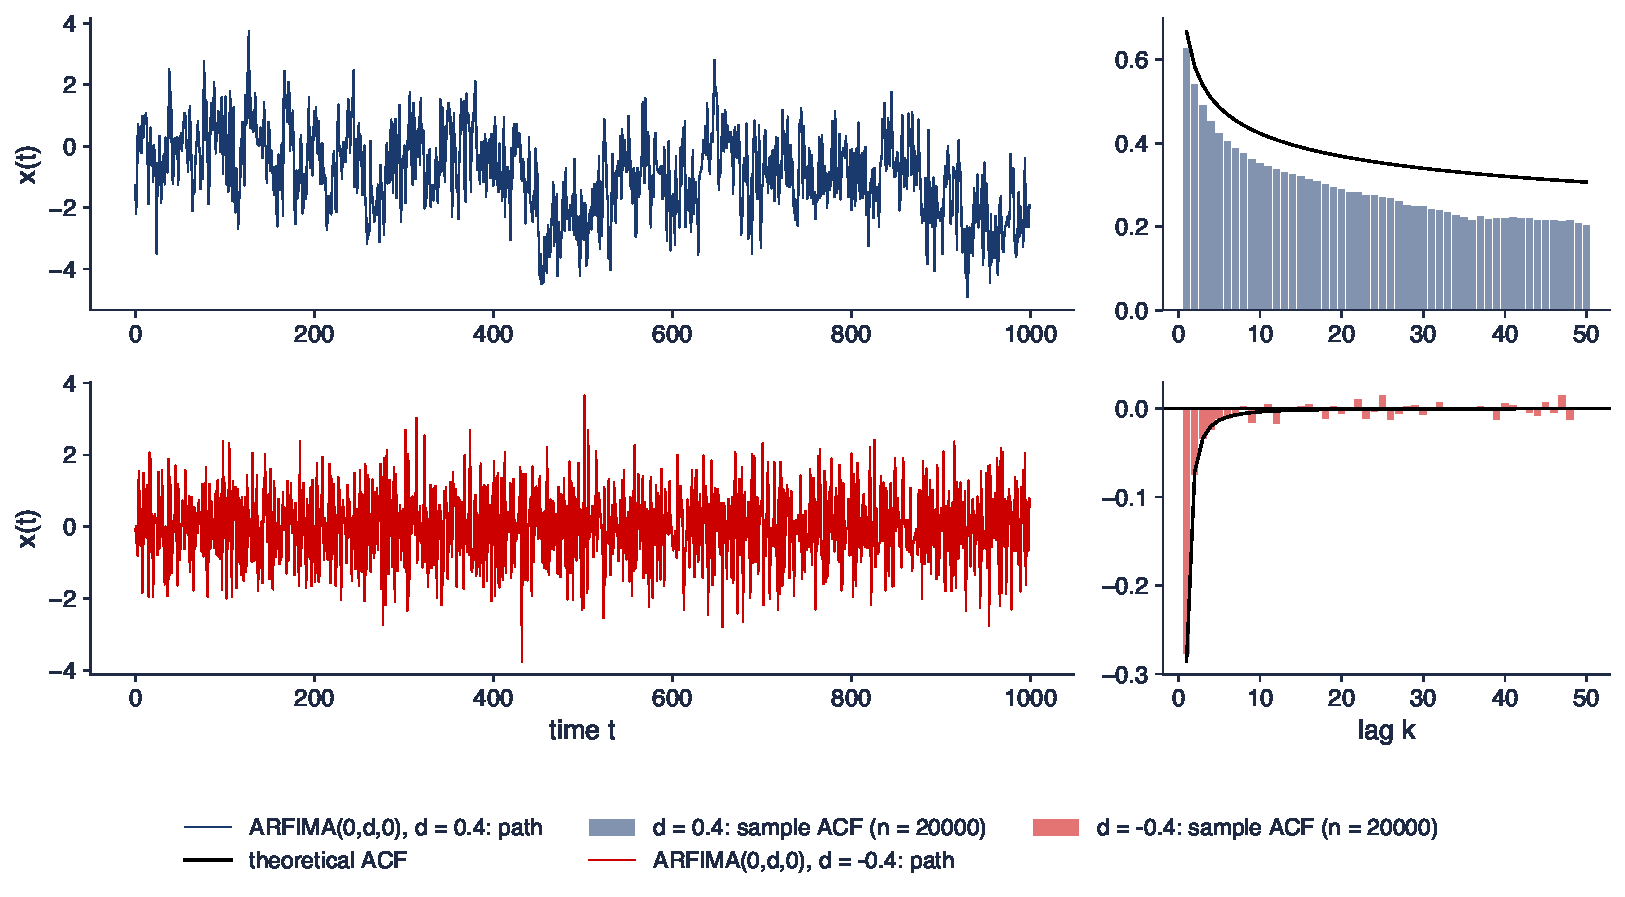
\includegraphics[width=0.97\textwidth,height=0.52\textheight,keepaspectratio]{sfm_ch11_arfima.pdf}
\end{center}
\vspace{-0.25cm}
\begin{itemize}
    \item Left: 1000 simulated values (as in SFEarfima); right: sample ACF (20000 values) and theoretical ACF
    \item $d = 0.4$: $\rho(1) = 0.667$, $\rho(10) = 0.424$, $\rho(50) = 0.307$: slow waves around the mean; $d = -0.4$: $\rho(1) = -0.286$, then almost zero
\end{itemize}
\sfmquantlet{Ch_11}{SFM_ch11_arfima}
\end{frame}

\begin{frame}{Worked Example: ARFIMA(0, 0.3, 0)}
\itemsize{\small}
\begin{itemize}
    \item Weights of $(1 - L)^{0.3}$: $\pi_1 = -d = -0.300$, $\pi_2 = \pi_1(1 - d)/2 = -0.105$
    \begin{itemize}
        \item MA weights: $\psi_1 = d = 0.300$, $\psi_2 = \psi_1(1 + d)/2 = 0.195$
    \end{itemize}
    \item Autocorrelations
    \begin{itemize}
        \item $\rho(1) = 0.3/0.7 = 0.429$; $\rho(2) = \rho(1) \times 1.3/1.7 = 0.328$
        \item $\rho(10) = 0.173$, $\rho(100) = 0.069$
    \end{itemize}
    \item AR(1) with $\phi = 0.429$: $\rho(10) = 0.0002$
    \item The autocorrelation falls below 0.05 after 4 lags for the AR(1) and after 222 lags for ARFIMA; $H = d + 0.5 = 0.8$
\end{itemize}
\end{frame}


%=============================================================================
\section{Estimators of Long Memory}
%=============================================================================

\begin{frame}{Four Tools}
\itemsize{\small}
\begin{center}
\scriptsize
\begin{tabular}{>{\raggedright\arraybackslash}p{2.0cm}>{\raggedright\arraybackslash}p{1.7cm}>{\raggedright\arraybackslash}p{3.4cm}>{\raggedright\arraybackslash}p{3.6cm}}
\toprule
\textbf{Tool} & \textbf{Domain} & \textbf{What it gives} & \textbf{Weak point} \\
\midrule
R/S & time & $\hat H$, slope of a log-log plot & biased upwards in small samples; sensitive to short memory \\
Lo's modified R/S & time & a test of short memory & low power against long memory \\
DFA & time & $\hat H$ (exponent $\alpha$) & needs block sizes; affected by breaks \\
GPH & frequency & $\hat d$ with a standard error & large variance; choice of bandwidth $m$ \\
\bottomrule
\end{tabular}
\end{center}
\begin{itemize}
    \item Other estimators: the local Whittle (Gaussian semiparametric) estimator \refRob, wavelets, exact maximum likelihood for ARFIMA (\refFHH, 14.5)
    \item Good practice: report several estimators, each with its uncertainty
\end{itemize}
\end{frame}

\begin{frame}{Detrended Fluctuation Analysis (DFA)}
\itemsize{\small}
\begin{itemize}
    \item \textbf{DFA} \refPeng: designed for signals with slowly changing trends
    \begin{itemize}
        \item 1. profile $Y_k = \sum_{j \le k}(x_j - \bar x)$
        \item 2. split $Y$ into blocks of size $n$; in each block, fit a straight line by OLS (linear detrending)
        \item 3. $F(n)$ = root mean square of the deviations from the lines, over all blocks
        \item 4. $F(n) \propto n^{\alpha}$: the slope of $\ln F(n)$ on $\ln n$ is $\hat\alpha$
    \end{itemize}
    \item Interpretation
    \begin{itemize}
        \item for fGn, $\alpha = H$: $\alpha = 0.5$ white noise, $0.5 < \alpha < 1$ long memory; for fBm, $\alpha = H + 1$
        \item the local line removes linear trends inside each block; $F(n)$ is unreliable for $n$ below about 10 \refKan
    \end{itemize}
\end{itemize}
\end{frame}

\begin{frame}{R/S and DFA: S\&P 500 since 2000}
\itemsize{\footnotesize}
\begin{center}
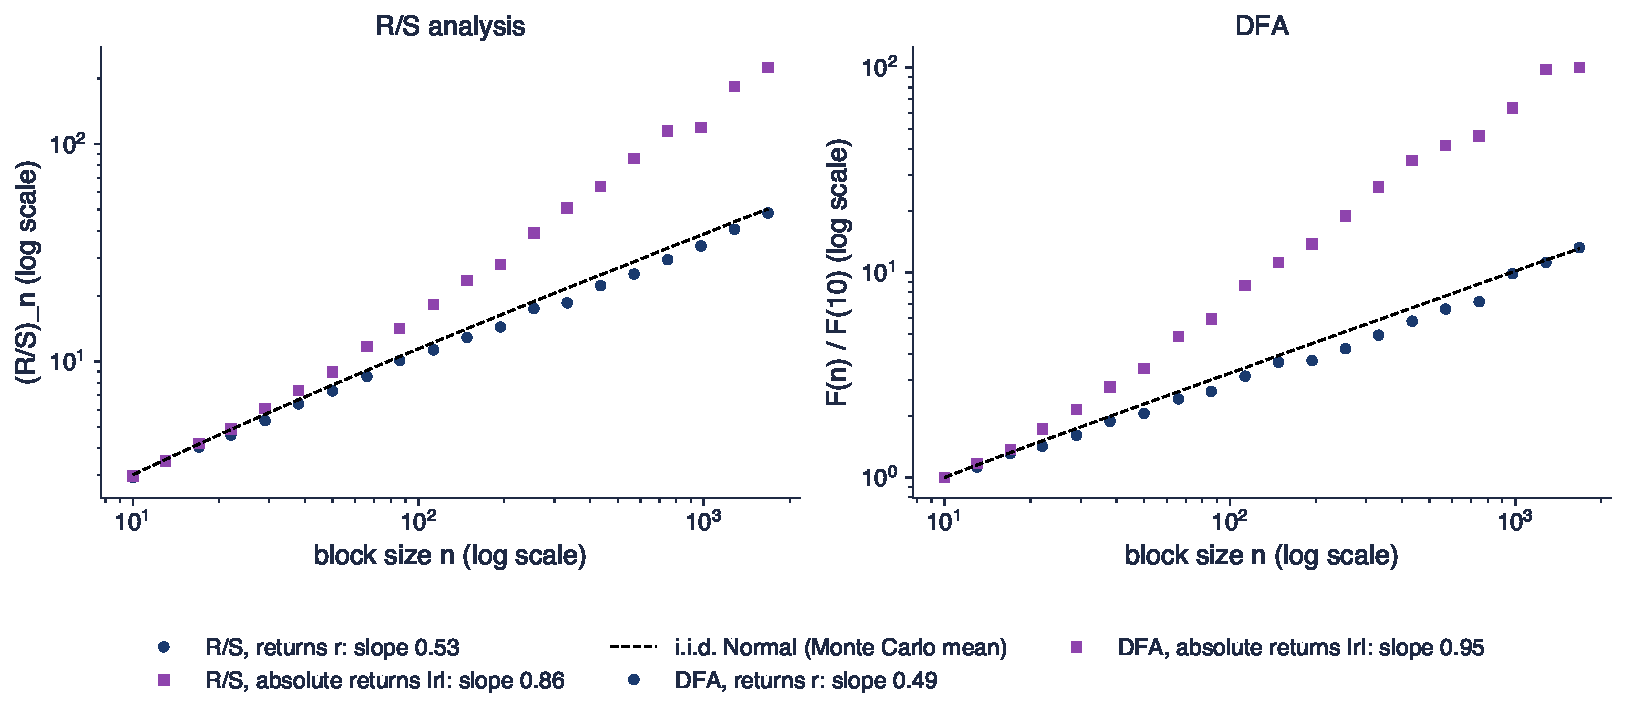
\includegraphics[width=0.97\textwidth,height=0.48\textheight,keepaspectratio]{sfm_ch11_rs_dfa.pdf}
\end{center}
\vspace{-0.25cm}
\begin{itemize}
    \item 20 block sizes from 10 to 1678 days; dashed: mean curve of i.i.d.\ Normal series of the same length
    \item Returns: R/S slope $0.53$ (i.i.d.\ series: $0.55$), DFA $0.49$ (i.i.d.: $0.50$): no long memory
    \item Absolute returns: R/S $0.86$, DFA $0.95$: strong long memory in volatility (Section 7)
\end{itemize}
\sfmquantlet{Ch_11}{SFM_ch11_rs_estimators}
\end{frame}

\begin{frame}{The GPH Log-Periodogram Regression}
\itemsize{\small}
\begin{itemize}
    \item \textbf{Periodogram} at the Fourier frequencies $\lambda_j = 2\pi j/T$: $I(\lambda_j) = \dfrac{1}{2\pi T}\left|\sum_{t=1}^{T} x_t e^{-i\lambda_j t}\right|^2$
    \begin{itemize}
        \item $T$: the number of observations; $i$: the imaginary unit; $|\cdot|^2$: the squared modulus
        \item it estimates the spectral density, which behaves like $C\lambda^{-2d}$ near zero
    \end{itemize}
    \item \textbf{GPH} \refGPH; \refFHH, 14.5.2: $\ln I(\lambda_j) = c - d\,\ln\!\left(4\sin^2(\lambda_j/2)\right) + e_j$, $j = 1, \dots, m$
    \begin{itemize}
        \item $m$: the number of low frequencies used; $c$: a constant; $e_j$: the error
        \item $\hat d$ = OLS slope on $-\ln(4\sin^2(\lambda_j/2))$; $\hat H = \hat d + 0.5$
        \item asymptotic standard error $\pi/\sqrt{24m}$; the bandwidth $m = \lfloor T^{0.5}\rfloor$
    \end{itemize}
    \item Trade-off: a small $m$ keeps only the long-run frequencies (small bias, large variance); a large $m$ lets short-run dynamics in (bias)
\end{itemize}
\end{frame}

\begin{frame}{GPH: S\&P 500 Returns and Absolute Returns}
\itemsize{\footnotesize}
\begin{center}
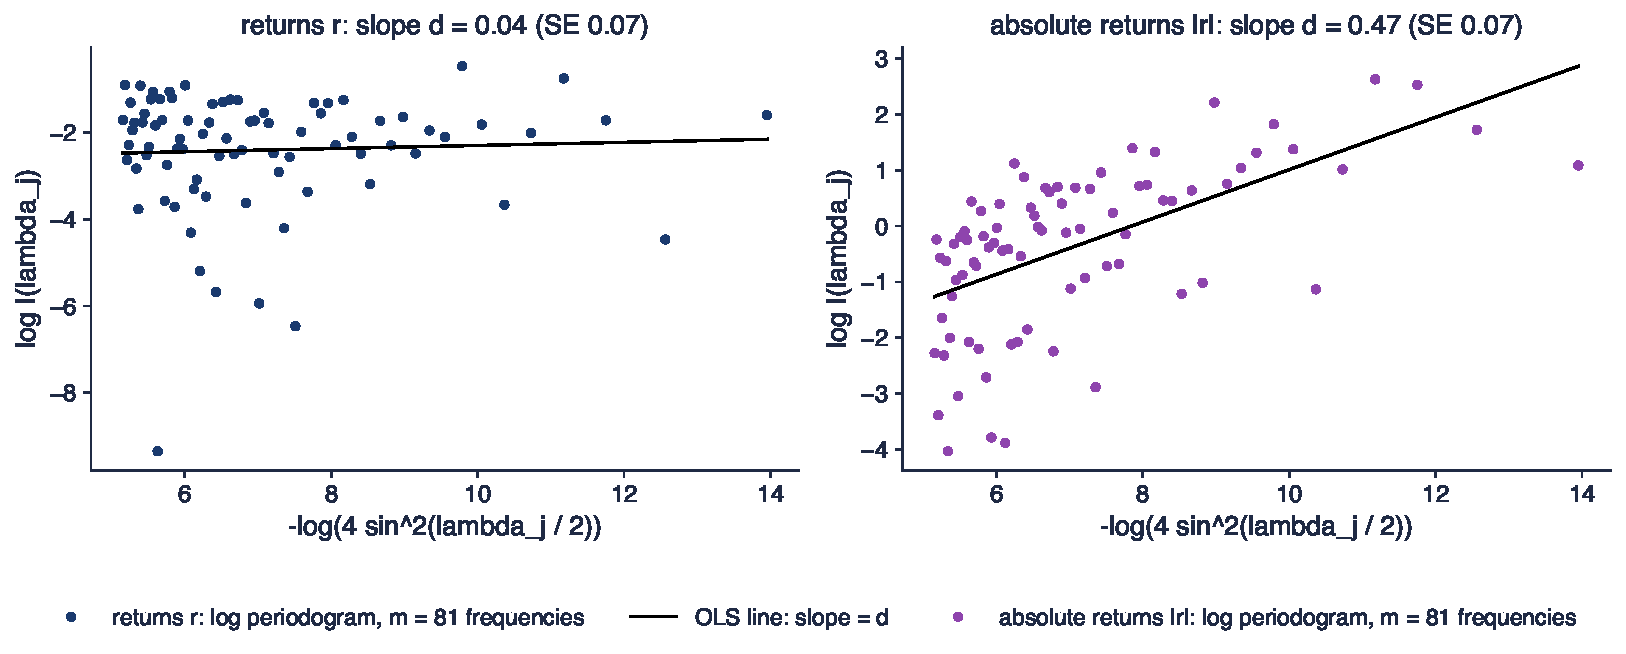
\includegraphics[width=0.97\textwidth,height=0.52\textheight,keepaspectratio]{sfm_ch11_gph.pdf}
\end{center}
\vspace{-0.25cm}
\begin{itemize}
    \item $m = 81$ lowest frequencies; each point is one frequency
    \item Returns: $\hat d = 0.036$ (SE $0.071$): not different from 0; absolute returns: $\hat d = 0.470$ (SE $0.071$), $\hat H = 0.97$
\end{itemize}
\sfmquantlet{Ch_11}{SFM_ch11_rs_estimators}
\end{frame}

\begin{frame}{Lo's Modified R/S Test}
\itemsize{\footnotesize}
\begin{itemize}
    \item Problem: short memory (e.g.\ an AR(1)) also raises R/S, so classical R/S mistakes short memory for long memory
    \item \refLo: $V_N(q) = \dfrac{R_N}{\sqrt{N}\,\hat\sigma_N(q)}$, $\hat\sigma^2_N(q) = \hat\gamma_0 + 2\sum_{j=1}^{q}\left(1 - \tfrac{j}{q + 1}\right)\hat\gamma_j$
    \begin{itemize}
        \item $N$: the number of returns; $R_N$: the range of the cumulative deviations over the whole sample
        \item $\hat\gamma_j$: sample autocovariances; $\hat\sigma^2_N(q)$: the Newey--West long-run variance \refNW; $q = 0$: classical R/S
        \item $q = \lfloor (3N/2)^{1/3}\,(2\hat\rho_1/(1 - \hat\rho_1^2))^{2/3}\rfloor$ ($\hat\rho_1$: first-order autocorrelation), data-dependent (Andrews' rule, used by Lo)
    \end{itemize}
    \item $H_0$: short memory; at 5\%, reject if $V_N(q) \notin [0.809, 1.862]$
    \begin{itemize}
        \item Lo's finding: no long memory in US stock index returns once short memory is allowed for
    \end{itemize}
\end{itemize}
\end{frame}

\begin{frame}{Classical against Modified R/S: Size and Power}
\itemsize{\footnotesize}
\begin{center}
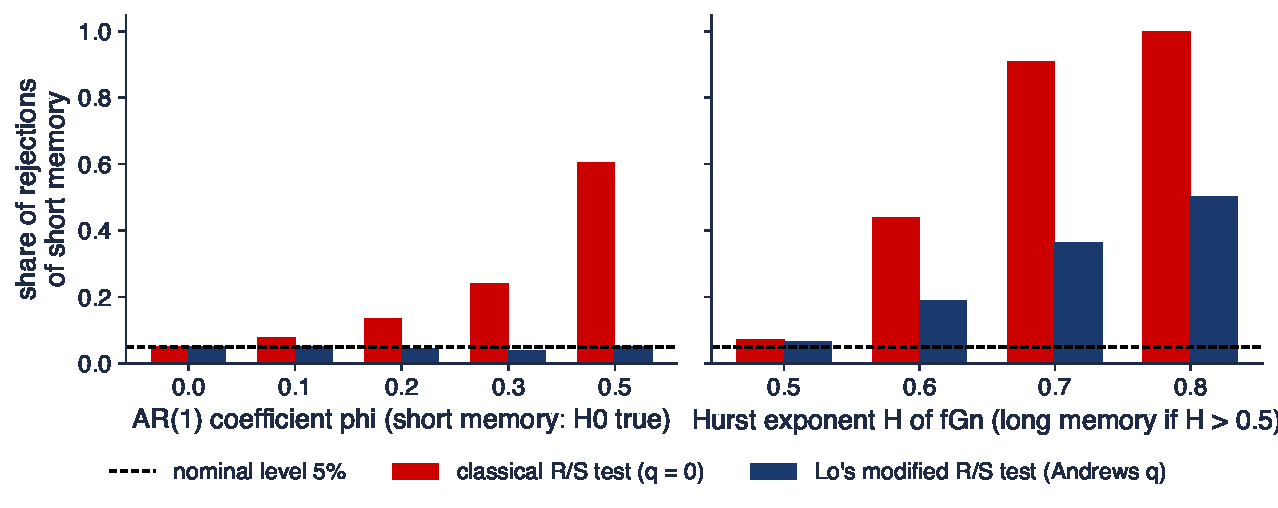
\includegraphics[width=0.97\textwidth,height=0.50\textheight,keepaspectratio]{sfm_ch11_lo_test.pdf}
\end{center}
\vspace{-0.25cm}
\begin{itemize}
    \item 500 series of 1000 values. Left, AR(1) (short memory, $H_0$ true): with $\phi = 0.5$ the classical test rejects in 60\% of cases, the modified test in 5\%
    \item Right, fGn (long memory if $H > 0.5$): with $H = 0.7$, rejection rates 91\% and 36\%: the correction costs power \refTTW
\end{itemize}
\sfmquantlet{Ch_11}{SFM_ch11_monte_carlo}
\end{frame}

\begin{frame}{Small Samples and Monte Carlo Bands}
\itemsize{\small}
\begin{itemize}
    \item Asymptotic results are unreliable for R/S and DFA at the sample sizes of finance; use simulation \refWeron
    \begin{itemize}
        \item 1. simulate many i.i.d.\ Normal series with the same length $N$ as the data
        \item 2. apply exactly the same estimator (same block sizes, same bandwidth)
        \item 3. the 2.5\% and 97.5\% quantiles of $\hat H$ form the 95\% band under $H = 0.5$
    \end{itemize}
    \item Reject $H = 0.5$ only if $\hat H$ lies outside the band
    \item i.i.d.\ Normal is the simplest null; a fitted short-memory model (AR, GARCH) gives a stricter null (Section 6)
\end{itemize}
\end{frame}

\begin{frame}{Monte Carlo: Bias and Spread of the Estimators}
\itemsize{\footnotesize}
\begin{center}
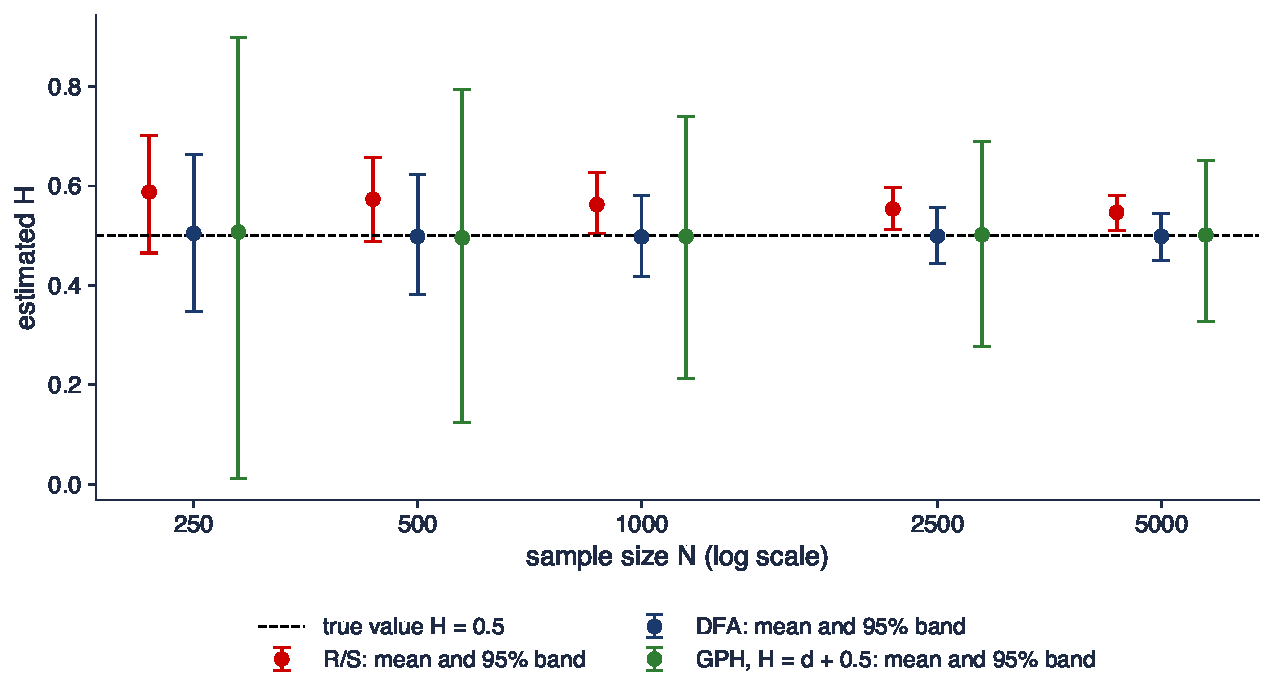
\includegraphics[width=0.97\textwidth,height=0.50\textheight,keepaspectratio]{sfm_ch11_mc_bias.pdf}
\end{center}
\vspace{-0.25cm}
\begin{itemize}
    \item 500 i.i.d.\ Normal series for each $N$; true $H = 0.5$
    \item R/S: mean $0.562$ at $N = 1000$ (biased upwards); DFA: $0.497$; GPH: $0.498$, unbiased but wide
    \item Width of the 95\% band at $N = 1000$: R/S $0.12$, DFA $0.16$, GPH $0.53$; at $N = 250$: DFA $0.32$
\end{itemize}
\sfmquantlet{Ch_11}{SFM_ch11_monte_carlo}
\end{frame}

\begin{frame}{S\&P 500: All Estimators}
\itemsize{\small}
\begin{center}
\footnotesize
\begin{tabular}{lrrrrr}
\toprule
 & R/S & DFA & GPH $\hat d$ (SE) & Lo $V_N(q)$ & $q$ \\
\midrule
returns $r_t$ & $0.53$ & $0.49$ & $0.04$ ($0.07$) & $1.56$ & 7 \\
absolute returns $|r_t|$ & $0.86$ & $0.95$ & $0.47$ ($0.07$) & $2.66$ & 15 \\
95\% band, i.i.d. & $[0.51, 0.57]$ & $[0.46, 0.54]$ & $[0.36, 0.65]$ & $[0.809, 1.862]$ &  \\
\bottomrule
\end{tabular}
\end{center}
\begin{itemize}
    \item $N = 6\,714$ daily returns, 2000 to 18 September 2026; GPH band given for $\hat H = \hat d + 0.5$
    \item Returns: every estimate inside its band, $V_N(q)$ inside $[0.809, 1.862]$
    \item Absolute returns: every estimate far above its band, Lo rejects short memory
\end{itemize}
\end{frame}

\begin{frame}{Interpretation: S\&P 500}
\itemsize{\small}
\begin{itemize}
    \item The direction of returns has no long memory since 2000
    \begin{itemize}
        \item consistent with the weak form of the EMH (\sfmchlink{https://danpele.github.io/SFM/EN/Courses/chapter7_efficient_markets_random_walk_vr.pdf}{Chapter 7}) and with \refLo
        \item R/S alone ($0.53$) would look like ``$H > 0.5$''; its band starts at $0.51$
    \end{itemize}
    \item The size of returns has long memory: $\hat d = 0.47$ for $|r_t|$
    \begin{itemize}
        \item the risk of a calm or turbulent period persists for months: the long-run version of volatility clustering
    \end{itemize}
    \item Before concluding ``long memory'', rule out spurious long memory: next section
\end{itemize}
\end{frame}


%=============================================================================
\section{Spurious Long Memory}
%=============================================================================

\begin{frame}{Breaks Look Like Memory}
\itemsize{\small}
\begin{itemize}
    \item A series with a few shifts in the mean has a sample ACF that decays slowly, like long memory
    \begin{itemize}
        \item two regimes with means $\mu_1 \neq \mu_2$: every pair of observations from the same regime shares the deviation $\mu_i - \bar x$
    \end{itemize}
    \item Landmark results
    \begin{itemize}
        \item \refDI: rare regime switches produce estimates of $d$ indistinguishable from true long memory
        \item \refGH: part of the long memory of S\&P 500 absolute returns comes from occasional breaks
        \item \refLS: long memory in squared S\&P 500 returns survives the checks; in returns, it is not found
    \end{itemize}
    \item Tests of true against spurious long memory: \refFHH, 14.4.3
\end{itemize}
\end{frame}

\begin{frame}{The Nile in 1898: a Break, Not Only Memory}
\itemsize{\footnotesize}
\begin{columns}[T]
\begin{column}{0.55\textwidth}
\begin{itemize}
    \item \refCobb: the annual flow of the Nile at Aswan, 1871--1970, changes its mean after 1898
    \item Mean flow: 1098 before, 850 after (in $10^8$ m$^3$), a drop of 23\%
    \item The change coincides with the building of the Aswan Low Dam (1898--1902)
    \item A river record with a break is the same problem as a market with a change of regime
\end{itemize}
\end{column}
\begin{column}{0.41\textwidth}
\centering
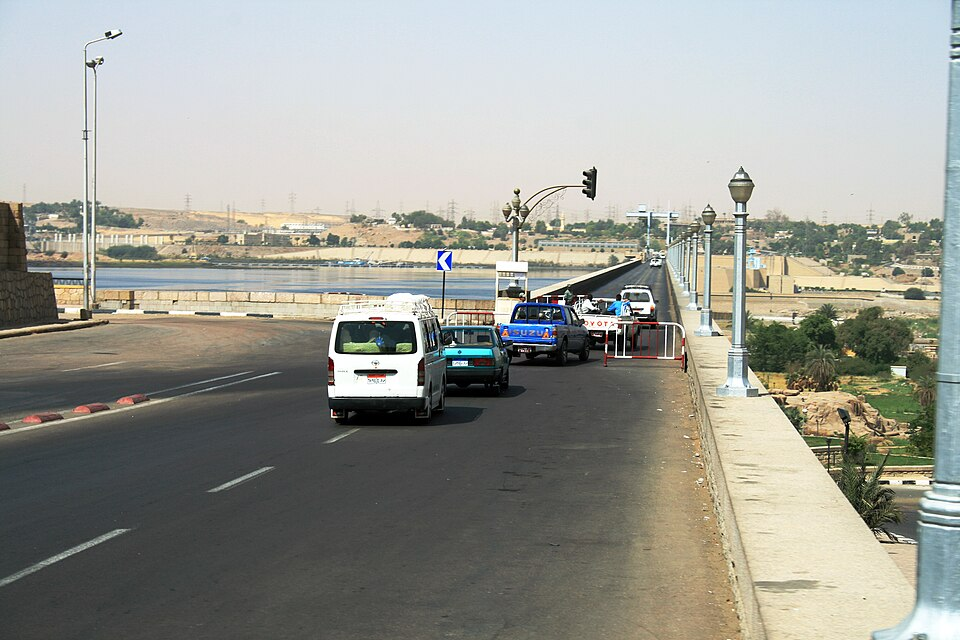
\includegraphics[height=0.36\textheight]{ch11_aswan_low_dam.jpg}\\[1mm]
\imgcap{The Aswan Low Dam on the Nile}
\imgcredit{https://commons.wikimedia.org/wiki/File:Aswan_Low_Dam_Egypt_1.jpg}{Photo: Karelj (2010); public domain; Wikimedia Commons}
\end{column}
\end{columns}
\end{frame}

\begin{frame}{The Nile: R/S before and after Removing the Break}
\itemsize{\footnotesize}
\begin{center}
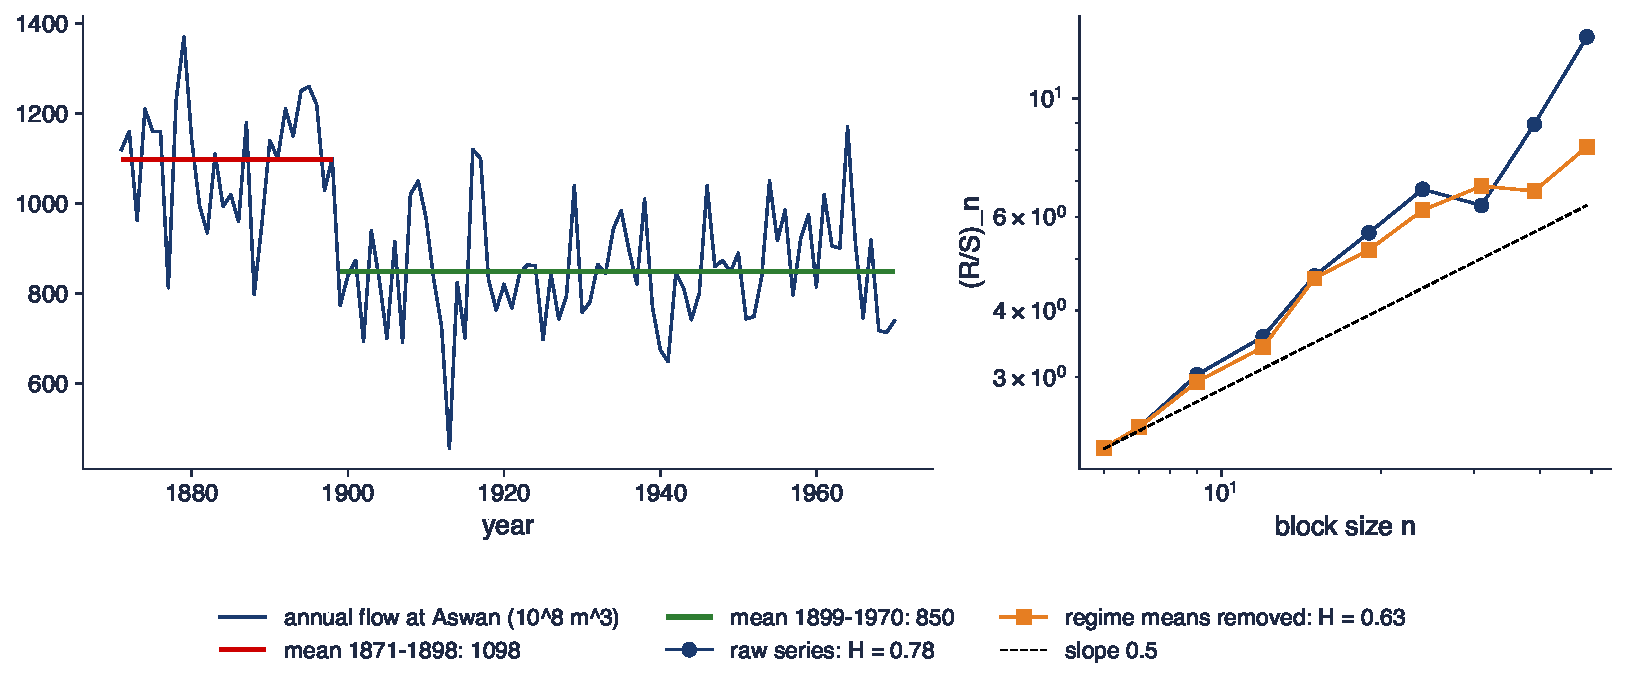
\includegraphics[width=0.97\textwidth,height=0.50\textheight,keepaspectratio]{sfm_ch11_nile.pdf}
\end{center}
\vspace{-0.25cm}
\begin{itemize}
    \item Raw series: $\hat H_{R/S} = 0.78$, DFA $0.84$; after removing the two regime means: $0.63$ and $0.50$
    \item With $N = 100$ the i.i.d.\ band for R/S is wide, $[0.45, 0.75]$, centred at $0.60$: most of the apparent memory was the break
\end{itemize}
\sfmquantlet{Ch_11}{SFM_ch11_spurious}
\end{frame}

\begin{frame}{Simulated Spurious Long Memory}
\itemsize{\footnotesize}
\begin{center}
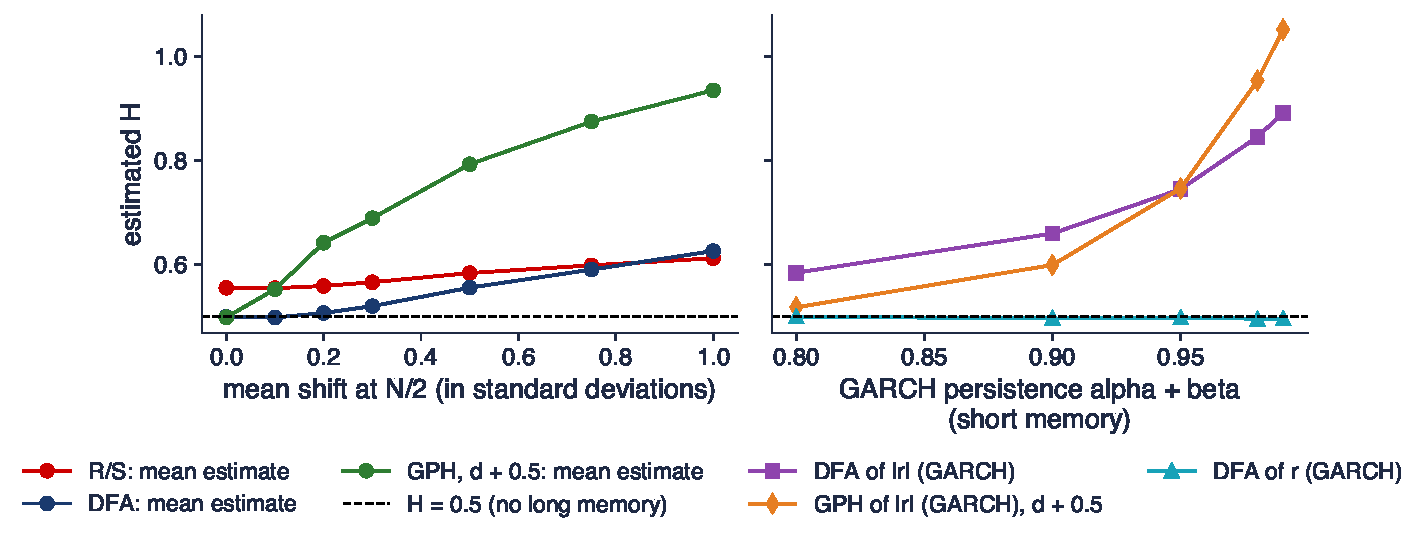
\includegraphics[width=0.97\textwidth,height=0.48\textheight,keepaspectratio]{sfm_ch11_spurious.pdf}
\end{center}
\vspace{-0.25cm}
\begin{itemize}
    \item 300 series of 2000 values. Left: i.i.d.\ $N(0,1)$ with a mean shift at the middle; a shift of 0.5 standard deviations gives GPH $\hat H = 0.79$, DFA $0.56$
    \item Right: GARCH(1,1), a short-memory model (\sfmchlink{https://danpele.github.io/SFM/EN/Courses/chapter9_arch_garch_models.pdf}{Chapter 9}); for $|r_t|$, DFA gives $0.74$ at $\alpha + \beta = 0.95$ and $0.89$ at $0.99$; the returns stay at $0.50$
\end{itemize}
\sfmquantlet{Ch_11}{SFM_ch11_spurious}
\end{frame}

\begin{frame}{Volatility Clustering Mimics Long Memory}
\itemsize{\small}
\begin{itemize}
    \item In GARCH(1,1), the ACF of $r_t^2$ decays like $(\alpha + \beta)^k$: short memory
    \begin{itemize}
        \item with $\alpha + \beta$ close to 1, the decay is so slow that a sample of a few thousand days cannot separate it from $k^{2d - 1}$
    \end{itemize}
    \item Consequence: a high $\hat H$ for $|r_t|$ is compatible with a persistent GARCH; it is not by itself proof of fractional dynamics
    \item For returns, GARCH does not create memory: the estimates stay at 0.5 (right panel)
    \item Better null hypothesis: simulate the fitted GARCH and compare $\hat H$ of the data with the GARCH band
\end{itemize}
\end{frame}

\begin{frame}{Checks against Spurious Long Memory}
\itemsize{\small}
\begin{itemize}
    \item \textbf{Shuffle test}: permute the series at random; the distribution stays, the order disappears; $\hat H$ should fall to 0.5
    \item \textbf{Subsamples}: estimate before and after known breaks (2008, 2020); true long memory appears in each subsample
    \item \textbf{Several estimators and bandwidths}: R/S, DFA, GPH with $m = T^{0.5}$ and $T^{0.6}$ should agree
    \item \textbf{Lo's modified R/S}: removes the effect of short memory
    \item \textbf{Model-based null}: Monte Carlo bands from a fitted AR or GARCH instead of i.i.d.\ noise
\end{itemize}
\end{frame}


%=============================================================================
\section{Long Memory in Volatility}
%=============================================================================

\begin{frame}{S\&P 500: the ACF of $r_t$, $|r_t|$ and $r_t^2$}
\itemsize{\footnotesize}
\begin{center}
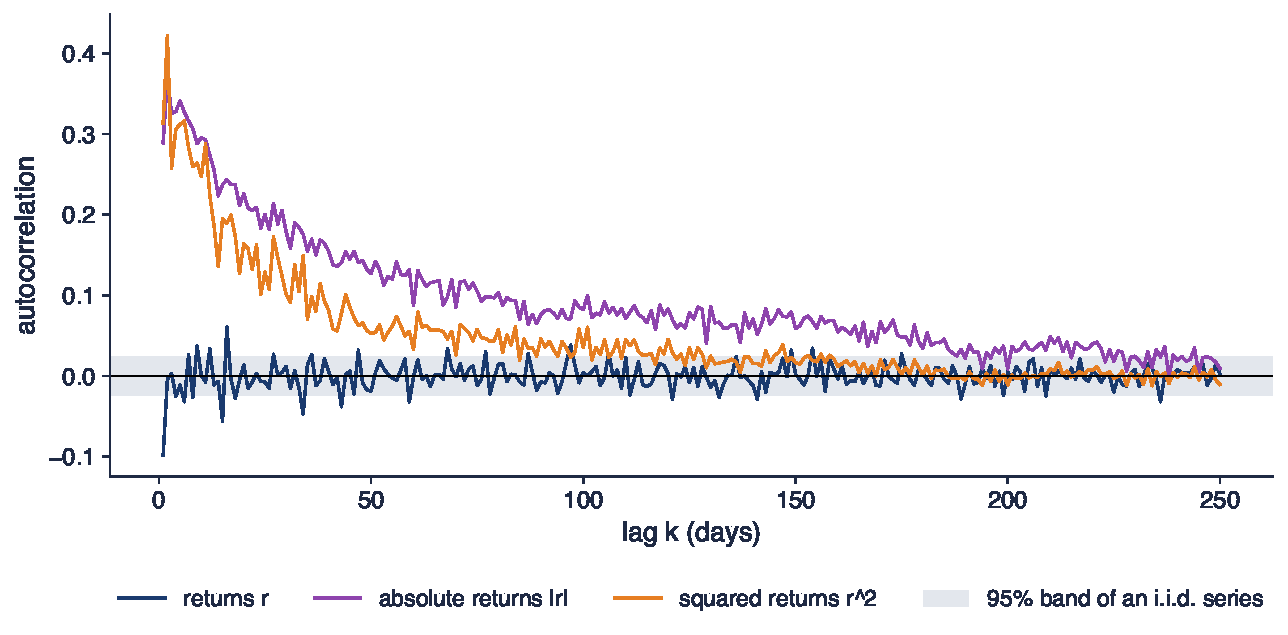
\includegraphics[width=0.97\textwidth,height=0.48\textheight,keepaspectratio]{sfm_ch11_vol_acf.pdf}
\end{center}
\vspace{-0.25cm}
\begin{itemize}
    \item $|r_t|$: $\rho(1) = 0.289$, $\rho(50) = 0.127$, $\rho(100) = 0.082$; 227 of the first 250 lags above the band $0.024$
    \item $r_t^2$: $\rho(1) = 0.313$, $\rho(50) = 0.053$; $r_t$: $\rho(1) = -0.099$, then inside the band
    \item \refDGE: $|r_t|$ is more persistent than $r_t^2$, which is more affected by single extreme days
\end{itemize}
\sfmquantlet{Ch_11}{SFM_ch11_volatility_memory}
\end{frame}

\begin{frame}{Six Markets: Returns and Absolute Returns}
\itemsize{\footnotesize}
\begin{center}
\scriptsize
\begin{tabular}{lrrrrrrrr}
\toprule
 & $N$ & \multicolumn{3}{c}{returns $r_t$} & \multicolumn{3}{c}{absolute returns $|r_t|$} & DFA band \\
 & & R/S & DFA & GPH $\hat d$ & DFA & GPH $\hat d$ & Lo $V$ &  \\
\midrule
S\&P 500 & 6\,714 & $0.53$ & $0.49$ & $0.04$ & $0.95$ & $0.47$ & $2.66$ & $[0.46, 0.54]$ \\
DAX & 6\,786 & $0.55$ & $0.50$ & $-0.06$ & $0.94$ & $0.48$ & $3.43$ & $[0.45, 0.54]$ \\
BET & 6\,670 & $0.58$ & $0.57$ & $0.17$ & $0.85$ & $0.47$ & $4.47$ & $[0.45, 0.54]$ \\
Bitcoin & 4\,384 & $0.59$ & $0.56$ & $0.05$ & $0.82$ & $0.33$ & $3.94$ & $[0.45, 0.55]$ \\
TLV & 3\,788 & $0.54$ & $0.47$ & $-0.06$ & $0.76$ & $0.25$ & $2.47$ & $[0.45, 0.55]$ \\
SNP & 3\,815 & $0.55$ & $0.49$ & $-0.02$ & $0.73$ & $0.21$ & $2.39$ & $[0.45, 0.55]$ \\
\bottomrule
\end{tabular}
\end{center}
\begin{itemize}
    \item Daily data to 18 September 2026: S\&P 500, DAX, BET since 2000, Bitcoin since 2014, TLV and SNP since 2010; standard error of GPH about $0.07$--$0.08$
    \item BET returns: DFA $0.57$ above its band, GPH $\hat d = 0.17$, Lo $V = 1.96$ rejects short memory
    \item Absolute returns: $\hat d$ from $0.21$ to $0.48$, Lo rejects for all six
\end{itemize}
\end{frame}

\begin{frame}{Six Markets: DFA Exponents and the Shuffle Test}
\itemsize{\footnotesize}
\begin{center}
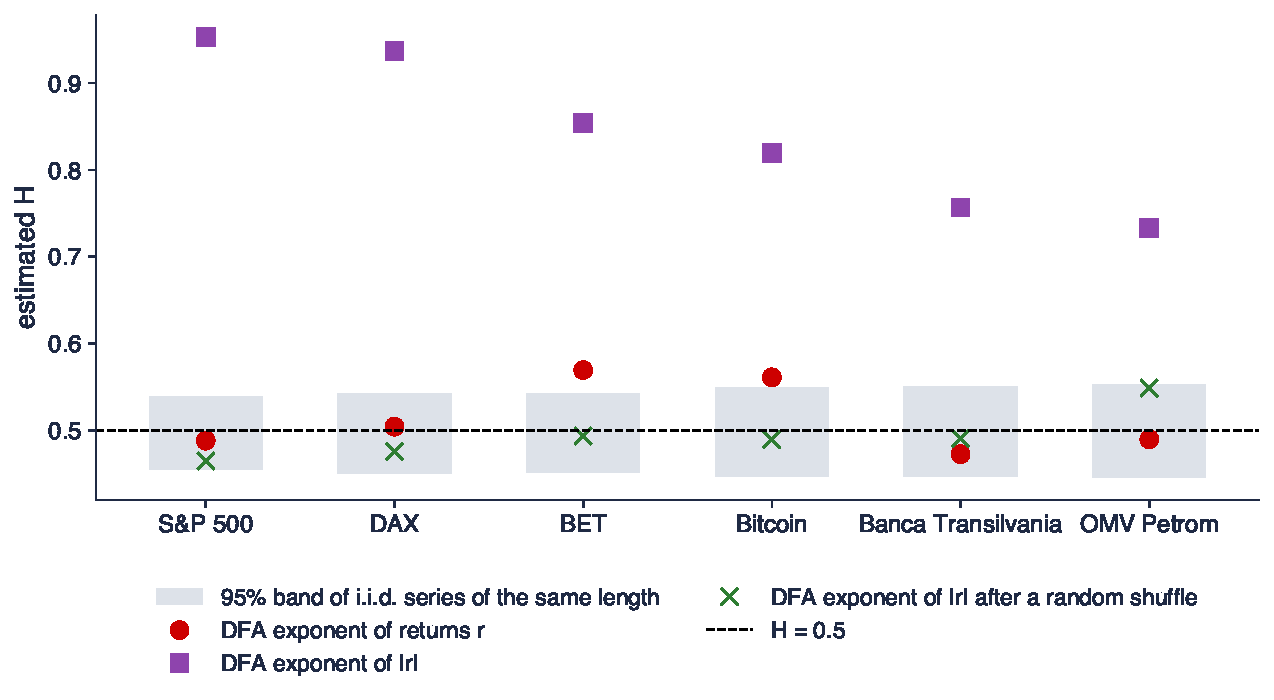
\includegraphics[width=0.97\textwidth,height=0.50\textheight,keepaspectratio]{sfm_ch11_markets.pdf}
\end{center}
\vspace{-0.25cm}
\begin{itemize}
    \item Shaded: 95\% band of i.i.d.\ series of the same length; circles: returns; squares: $|r_t|$; crosses: $|r_t|$ after a random shuffle
    \item $|r_t|$: DFA from $0.73$ to $0.95$; after shuffling: from $0.46$ to $0.55$, inside the bands: the memory lies in the order of the days
\end{itemize}
\sfmquantlet{Ch_11}{SFM_ch11_volatility_memory}
\end{frame}

\begin{frame}{Interpretation: What Is Predictable?}
\itemsize{\small}
\begin{itemize}
    \item \textbf{Returns}: no long memory in the S\&P 500, DAX, TLV and SNP; Bitcoin at the edge of its band
    \begin{itemize}
        \item BET: persistence, as in the variance-ratio tests of \sfmchlink{https://danpele.github.io/SFM/EN/Courses/chapter7_efficient_markets_random_walk_vr.pdf}{Chapter 7}; partly the thin trading of the early years (Section 8)
    \end{itemize}
    \item \textbf{Volatility}: long memory everywhere, strongest in the large equity indices
    \begin{itemize}
        \item the risk regime of today is informative for months: useful for VaR (value at risk) and option pricing
    \end{itemize}
    \item Weak-form efficiency (unpredictable direction) and predictable risk coexist: the FMH adds a reason, investors with different horizons react to volatility on different time scales
\end{itemize}
\end{frame}

\begin{frame}{Models for Long Memory in Volatility}
\itemsize{\small}
\begin{itemize}
    \item \textbf{FIGARCH} (fractionally integrated GARCH) \refBBM; \refFHH, 14.6.2: $(1 - L)^d$ applied to $\varepsilon_t^2$
    \begin{itemize}
        \item shocks to volatility decay hyperbolically; $d = 0$ gives GARCH, $d = 1$ gives IGARCH (integrated GARCH, \sfmchlink{https://danpele.github.io/SFM/EN/Courses/chapter9_arch_garch_models.pdf}{Chapter 9})
    \end{itemize}
    \item \textbf{Heterogeneous horizons}, the FMH idea in volatility models
    \begin{itemize}
        \item \refMuller: market components with different time resolutions (intraday traders to long-term investors)
        \item \refAB: many volatility components with different persistence add up to long memory
        \item \refCorsi: HAR (heterogeneous autoregressive) model, tomorrow's volatility on the daily, weekly and monthly volatility: three horizons, approximate long memory
    \end{itemize}
\end{itemize}
\end{frame}


%=============================================================================
\section{Rolling Hurst Exponents}
%=============================================================================

\begin{frame}{Does Efficiency Change over Time?}
\itemsize{\small}
\begin{itemize}
    \item The AMH and the FMH both predict that market memory changes over time
    \begin{itemize}
        \item \refCT: rolling Hurst exponents of emerging stock markets, to test whether they become more efficient
        \item \refBar: rolling DFA on Bitcoin returns and volatility
    \end{itemize}
    \item Design used here
    \begin{itemize}
        \item windows of 1000 observations (about four years of trading days), moved by 21 observations (about one month)
        \item DFA on $r_t$ and on $|r_t|$; each estimate dated at the last day of its window, so it uses only past data
        \item 95\% Monte Carlo band for $N = 1000$: $[0.42, 0.58]$
    \end{itemize}
\end{itemize}
\end{frame}

\begin{frame}{Rolling DFA Exponents: S\&P 500, BET, Bitcoin}
\itemsize{\footnotesize}
\begin{center}
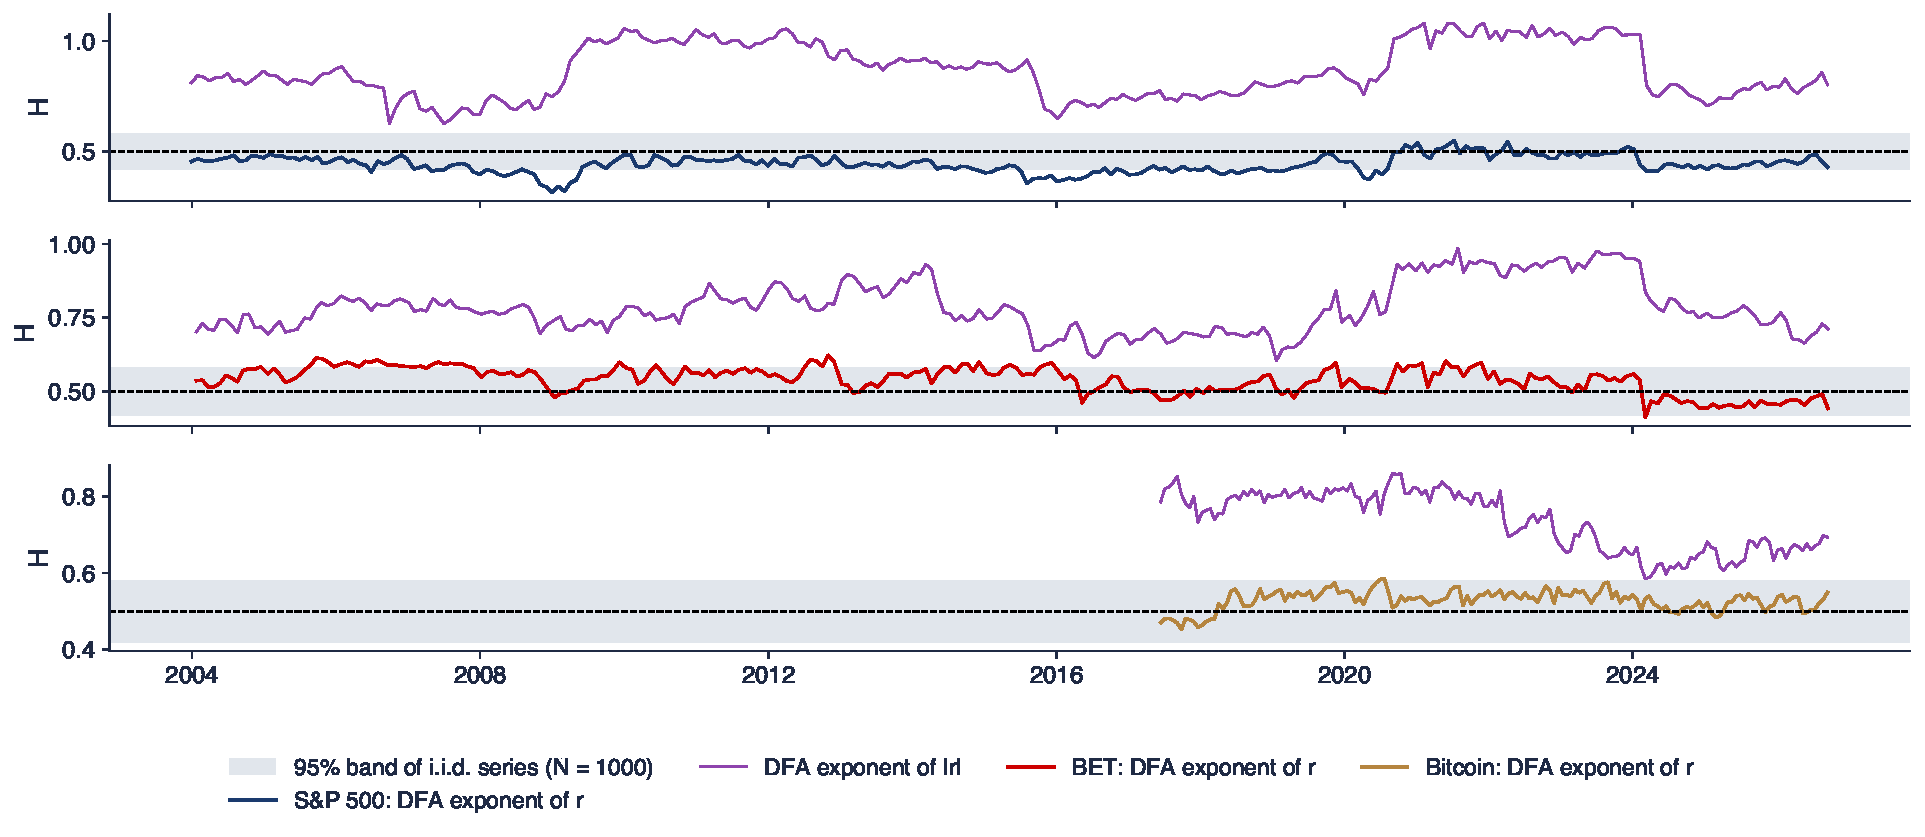
\includegraphics[width=0.97\textwidth,height=0.60\textheight,keepaspectratio]{sfm_ch11_rolling.pdf}
\end{center}
\vspace{-0.25cm}
\begin{itemize}
    \item Top to bottom: S\&P 500, BET, Bitcoin; coloured line: $r_t$; purple line: $|r_t|$; shaded: i.i.d.\ band
    \item $|r_t|$ always far above the band; its exponent rises in and after crises (2008--2009, 2020)
\end{itemize}
\sfmquantlet{Ch_11}{SFM_ch11_rolling_hurst}
\end{frame}

\begin{frame}{Interpretation: Rolling Exponents}
\itemsize{\small}
\begin{itemize}
    \item S\&P 500: 273 windows; $\hat H$ of returns between $0.32$ and $0.55$; 24\% of windows below the band, none above
    \begin{itemize}
        \item the minimum, 31 December 2008, follows the 2008 crash: daily reversals (anti-persistence) in a panic
    \end{itemize}
    \item BET: 20\% of windows above the band; mean $\hat H$ $0.56$ in the first third of the windows, $0.52$ in the last third
    \begin{itemize}
        \item the maximum, 31 October 2012; a market that becomes more efficient as liquidity grows
    \end{itemize}
    \item Bitcoin: windows from 13 June 2017; $\hat H$ between $0.45$ and $0.59$, 1\% of windows above the band
\end{itemize}
\end{frame}

\begin{frame}{Case Study: Is Bitcoin Efficient?}
\itemsize{\footnotesize}
\begin{columns}[T]
\begin{column}{0.60\textwidth}
\begin{itemize}
    \item \refUrq: several tests, among them R/S, on Bitcoin 2010--2016
    \begin{itemize}
        \item inefficient over the full sample, moving towards efficiency in the later years
    \end{itemize}
    \item \refNC: the same data after a power transformation of the returns: consistent with weak-form efficiency
    \item \refBar: rolling DFA: persistent returns until 2014, close to $H = 0.5$ afterwards; long memory in volatility throughout
    \item Our windows start in 2017 and agree: returns near the band, $|r_t|$ far above it
\end{itemize}
\end{column}
\begin{column}{0.36\textwidth}
\centering
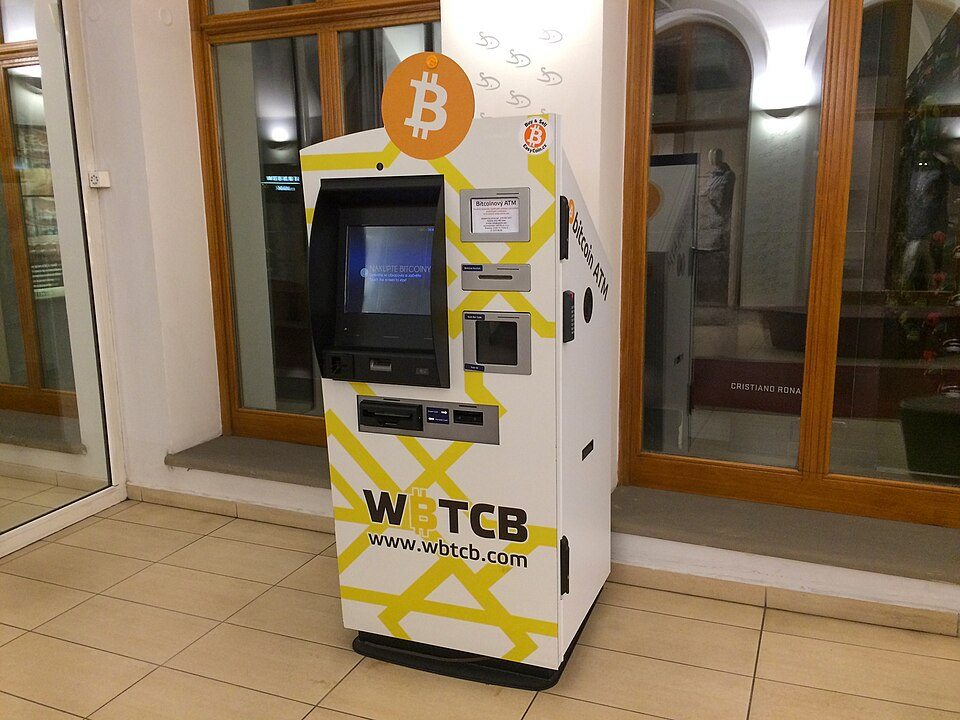
\includegraphics[height=0.40\textheight]{ch11_bitcoin_atm_prague.jpg}\\[1mm]
\imgcap{A Bitcoin cash machine in Prague (2016)}
\imgcredit{https://commons.wikimedia.org/wiki/File:Bitcoin_ATM_Prague.jpg}{Photo: Perituss (2016); CC0; Wikimedia Commons}
\end{column}
\end{columns}
\end{frame}

\begin{frame}{Pitfalls of Rolling Estimates}
\itemsize{\small}
\begin{itemize}
    \item \textbf{Multiple testing}: 273 windows at 5\% each give about 14 windows outside the band by chance
    \begin{itemize}
        \item look for long runs outside the band, not for isolated windows
    \end{itemize}
    \item \textbf{Overlap}: consecutive windows share 979 of their 1000 observations; the path is smooth by construction
    \item \textbf{Window length}: shorter windows react faster but have wider bands (DFA, $N = 250$: width $0.32$)
    \item \textbf{Volatility regimes}: a crisis inside a window shifts the estimate for four years
    \item \textbf{Dating}: date each estimate at the end of its window, never at the middle (no look-ahead)
\end{itemize}
\end{frame}


%=============================================================================
\section{Long Memory and Risk}
%=============================================================================

\begin{frame}{Scaling Risk with $h^H$}
\itemsize{\footnotesize}
\begin{itemize}
    \item If returns are self-similar: $h$-day VaR 1\% $= -z_{0.01}\,\sigma\,h^H$, with $z_{0.01} = -2.326$ (Normal case, mean 0)
    \begin{itemize}
        \item $z_{0.01}$: the 1\% quantile of $N(0,1)$; $\sigma$: the daily volatility; $h^H$ replaces the factor $\sqrt{h}$
        \item daily volatility $\sigma = 1.2\%$: one-day VaR 1\% $= 2.79\%$
    \end{itemize}
    \item Ten days
    \begin{itemize}
        \item $H = 0.45$: factor $2.82$, VaR $7.87\%$; $H = 0.5$: $3.16$, $8.83\%$; $H = 0.55$: $3.55$, $9.90\%$
        \item $H = 0.55$ instead of 0.5: 12\% more risk at 10 days, 32\% more at 250 days
    \end{itemize}
    \item Data: the 10-day ratio is $2.80$ for the S\&P 500 and $3.50$ for the BET, against $\sqrt{10} = 3.16$: the $\sqrt{h}$ rule overstates S\&P 500 risk and understates BET risk (\sfmchlink{https://danpele.github.io/SFM/EN/Courses/chapter10_var_es_backtesting.pdf}{Chapter 10})
    \item Pricing: with fBm prices and $H \neq 1/2$, a frictionless market admits arbitrage \refRogers; long memory enters option models through volatility instead
\end{itemize}
\end{frame}


%=============================================================================
\section{AI for Scientific Discovery}
%=============================================================================

\begin{frame}{An Open Question}
\itemsize{\small}
\begin{itemize}
    \item \textbf{Does a change in the Hurst exponent come before a crisis, or only after it?}
    \begin{itemize}
        \item the FMH predicts a collapse of horizons; in our data, $\hat H$ of $|r_t|$ rises in and after 2008 and 2020
        \item a rolling window contains the crisis only after it starts: is there any signal before?
    \end{itemize}
    \item Earlier evidence: \refKrisB\ (horizons in 2008); \refCT\ (emerging markets)
    \item Why it is open: few crises, overlapping windows, volatility regimes, many possible estimators
    \item AI tools can speed up such a study, but its results must still be checked \refWang
\end{itemize}
\end{frame}

\begin{frame}{How AI Could Help}
\itemsize{\small}
\begin{itemize}
    \item \textbf{Literature}: a list of studies on Hurst exponents as early-warning indicators, with their data and estimators
    \item \textbf{Code}: a first draft of rolling R/S, DFA and GPH with Monte Carlo bands
    \item \textbf{Robustness}: other window lengths, wavelet estimators, a GARCH-based null, other crises (2011, 2022)
    \item Example prompt
    \begin{itemize}
        \item \aiprompt{Write Python code that computes the DFA exponent of daily S\&P 500 absolute log returns on rolling windows of 500 and 1000 days, dated at the window end, adds a 95\% band from 500 simulated GARCH(1,1) paths, and marks the start of the 2008 and 2020 crises.}
    \end{itemize}
\end{itemize}
\end{frame}

\begin{frame}{What to Check}
\itemsize{\small}
\begin{itemize}
    \item Dating: an estimate dated at the middle of its window uses future data
    \item Conversions: $d = H - 0.5$, not $H + 0.5$; DFA on prices gives $H + 1$, not $H$
    \item Bands: every $\hat H$ needs a band for its own $N$; R/S is biased upwards
    \item Returns or volatility: memory in $|r_t|$ does not make the direction of returns predictable
    \item GPH bandwidth: $m = T/2$ (all frequencies) is not ``more accurate''; report $T^{0.5}$ and $T^{0.6}$
    \item References: every cited paper must exist; check the DOI
\end{itemize}
\end{frame}

\begin{frame}{Project Idea}
\itemsize{\small}
\begin{itemize}
    \item \textbf{Question}: does the rolling Hurst exponent of volatility rise before crises on the BVB and in Bitcoin?
    \begin{itemize}
        \item data: BET, BET-TR, TLV, SNP and Bitcoin (EODHD), daily
    \end{itemize}
    \item Steps
    \begin{itemize}
        \item rolling DFA and GPH of $r_t$ and $|r_t|$, windows of 500 and 1000 days, dated at the end
        \item bands from i.i.d.\ and from fitted GARCH(1,1) simulations
        \item event windows around 2008, 2020 and 2022: the exponent in the 60 days before and after
    \end{itemize}
    \item Deliverable: one table, one chart, and a paragraph on what the data can and cannot show
    \item Declare any AI use, and list the errors of the AI that you corrected
\end{itemize}
\end{frame}


%=============================================================================
\section{Summary}
%=============================================================================

\begin{frame}{Key Takeaways}
\itemsize{\small}
\begin{itemize}
    \item FMH: stability needs investors with many horizons; crises are collapses of horizons
    \item $H$ measures memory and scaling: $H = 0.5$ none, $H > 0.5$ persistence, $H < 0.5$ anti-persistence; $d = H - 0.5$
    \item R/S, DFA, GPH and Lo's test, always with a Monte Carlo band for the same $N$
    \item Breaks and persistent GARCH volatility create spurious long memory: shuffle, split, compare
    \item Returns: no long memory in large markets (BET: persistence); volatility: long memory everywhere
    \item Multi-day risk scales like $h^H$
\end{itemize}
\end{frame}

\begin{frame}{Key Formulas}
\itemsize{\small}
{\renewcommand{\arraystretch}{1.45}\begin{center}
\small
\begin{tabular}{ll}
\toprule
\textbf{Quantity} & \textbf{Formula} \\
\midrule
Self-similarity & $X_{ct} \overset{d}{=} c^H X_t$; \quad $\mathrm{sd}(r^{(h)}) = h^H \mathrm{sd}(r)$ \\
R/S & $(R/S)_n = \left[\max_k Y_k - \min_k Y_k\right]/S_n$, \quad $Y_k = \sum_{j \le k}(x_j - \bar x)$; \quad $(R/S)_n \propto n^H$ \\
fGn & $\rho(k) = \tfrac12(|k + 1|^{2H} - 2|k|^{2H} + |k - 1|^{2H}) \approx H(2H - 1)k^{2H - 2}$ \\
ARFIMA(0,$d$,0) & $(1 - L)^d X_t = \varepsilon_t$, \quad $\rho(k) = \rho(k - 1)\frac{k - 1 + d}{k - d}$, \quad $d = H - 0.5$ \\
DFA & $F(n) \propto n^{\alpha}$, \quad $\alpha = H$ for fGn \\
GPH & $\ln I(\lambda_j) = c - d\ln(4\sin^2(\lambda_j/2)) + e_j$, \quad $j \le m = T^{0.5}$, \quad SE $= \pi/\sqrt{24m}$ \\
Lo & $V_N(q) = R_N/(\sqrt{N}\hat\sigma_N(q))$; reject at 5\% outside $[0.809, 1.862]$ \\
VaR 1\% & $-z_{0.01}\,\sigma\,h^H$ \\
\bottomrule
\end{tabular}
\end{center}
}
\end{frame}

\begin{frame}{Check Yourself}
\itemsize{\footnotesize}
\begin{itemize}
    \item \textbf{Question}: an R/S estimate on 1000 i.i.d.\ returns is $\hat H = 0.56$. Is this evidence of long memory?
    \begin{itemize}
        \item \textbf{Answer}: no: the i.i.d.\ band for $N = 1000$ is $[0.50, 0.63]$, centred near $0.562$
    \end{itemize}
    \item \textbf{Question}: GPH gives $\hat d = 0.35$ for $|r_t|$. What is $\hat H$?
    \begin{itemize}
        \item \textbf{Answer}: $\hat H = \hat d + 0.5 = 0.85$: long memory in volatility, not in returns
    \end{itemize}
    \item \textbf{Question}: after a random shuffle of $|r_t|$, DFA falls from 0.9 to 0.5. What does this show?
    \begin{itemize}
        \item \textbf{Answer}: the memory comes from the order of the days, not from the distribution (heavy tails)
    \end{itemize}
    \item Next: \sfmchlink{https://danpele.github.io/SFM/EN/Courses/chapter12_scoring_models.pdf}{Chapter 12}, scoring models
\end{itemize}
\end{frame}


%=============================================================================
\section{References}
%=============================================================================

\begin{frame}{References (1/3)}
\itemsize{\tiny}
\begin{itemize}
    \item Andersen, T.G., Bollerslev, T. (1997). \href{https://doi.org/10.1111/j.1540-6261.1997.tb02722.x}{Heterogeneous information arrivals and return volatility dynamics: uncovering the long-run in high frequency returns}. \textit{Journal of Finance}, 52(3), 975--1005.
    \item Anis, A.A., Lloyd, E.H. (1976). \href{https://doi.org/10.1093/biomet/63.1.111}{The expected value of the adjusted rescaled Hurst range of independent normal summands}. \textit{Biometrika}, 63(1), 111--116.
    \item Baillie, R.T. (1996). \href{https://doi.org/10.1016/0304-4076(95)01732-1}{Long memory processes and fractional integration in econometrics}. \textit{Journal of Econometrics}, 73(1), 5--59.
    \item Baillie, R.T., Bollerslev, T., Mikkelsen, H.O. (1996). \href{https://doi.org/10.1016/S0304-4076(95)01749-6}{Fractionally integrated generalized autoregressive conditional heteroskedasticity}. \textit{Journal of Econometrics}, 74(1), 3--30.
    \item Bariviera, A.F. (2017). \href{https://doi.org/10.1016/j.econlet.2017.09.013}{The inefficiency of Bitcoin revisited: a dynamic approach}. \textit{Economics Letters}, 161, 1--4.
    \item Cajueiro, D.O., Tabak, B.M. (2004). \href{https://doi.org/10.1016/j.physa.2003.12.031}{The Hurst exponent over time: testing the assertion that emerging markets are becoming more efficient}. \textit{Physica A}, 336(3--4), 521--537.
    \item Carlson, M. (2007). \href{https://www.federalreserve.gov/pubs/feds/2007/200713/index.html}{A brief history of the 1987 stock market crash with a discussion of the Federal Reserve response}. Finance and Economics Discussion Series 2007-13, Federal Reserve Board.
    \item Cobb, G.W. (1978). \href{https://doi.org/10.1093/biomet/65.2.243}{The problem of the Nile: conditional solution to a changepoint problem}. \textit{Biometrika}, 65(2), 243--251.
    \item Corsi, F. (2009). \href{https://doi.org/10.1093/jjfinec/nbp001}{A simple approximate long-memory model of realized volatility}. \textit{Journal of Financial Econometrics}, 7(2), 174--196.
    \item Diebold, F.X., Inoue, A. (2001). \href{https://doi.org/10.1016/S0304-4076(01)00073-2}{Long memory and regime switching}. \textit{Journal of Econometrics}, 105(1), 131--159.
    \item Ding, Z., Granger, C.W.J., Engle, R.F. (1993). \href{https://doi.org/10.1016/0927-5398(93)90006-D}{A long memory property of stock market returns and a new model}. \textit{Journal of Empirical Finance}, 1(1), 83--106.
    \item Fama, E.F. (1970). \href{https://doi.org/10.2307/2325486}{Efficient capital markets: a review of theory and empirical work}. \textit{Journal of Finance}, 25(2), 383--417.
    \item Franke, J., Härdle, W.K., Hafner, C.M. (2019). \href{https://doi.org/10.1007/978-3-030-13751-9}{\textit{Statistics of Financial Markets: An Introduction}}, 5th ed. Springer.
    \item Geweke, J., Porter-Hudak, S. (1983). \href{https://doi.org/10.1111/j.1467-9892.1983.tb00371.x}{The estimation and application of long memory time series models}. \textit{Journal of Time Series Analysis}, 4(4), 221--238.
\end{itemize}
\end{frame}

\begin{frame}{References (2/3)}
\itemsize{\tiny}
\begin{itemize}
    \item Granger, C.W.J., Hyung, N. (2004). \href{https://doi.org/10.1016/j.jempfin.2003.03.001}{Occasional structural breaks and long memory with an application to the S\&P 500 absolute stock returns}. \textit{Journal of Empirical Finance}, 11(3), 399--421.
    \item Granger, C.W.J., Joyeux, R. (1980). \href{https://doi.org/10.1111/j.1467-9892.1980.tb00297.x}{An introduction to long-memory time series models and fractional differencing}. \textit{Journal of Time Series Analysis}, 1(1), 15--29.
    \item Hosking, J.R.M. (1981). \href{https://doi.org/10.1093/biomet/68.1.165}{Fractional differencing}. \textit{Biometrika}, 68(1), 165--176.
    \item Hurst, H.E. (1951). \href{https://doi.org/10.1061/TACEAT.0006518}{Long-term storage capacity of reservoirs}. \textit{Transactions of the American Society of Civil Engineers}, 116(1), 770--799.
    \item Kantelhardt, J.W., Koscielny-Bunde, E., Rego, H.H.A., Havlin, S., Bunde, A. (2001). \href{https://doi.org/10.1016/S0378-4371(01)00144-3}{Detecting long-range correlations with detrended fluctuation analysis}. \textit{Physica A}, 295(3--4), 441--454.
    \item Kristoufek, L. (2012). \href{https://doi.org/10.1142/S0219525912500658}{Fractal markets hypothesis and the global financial crisis: scaling, investment horizons and liquidity}. \textit{Advances in Complex Systems}, 15(6), 1250065.
    \item Kristoufek, L. (2013). \href{https://doi.org/10.1038/srep02857}{Fractal markets hypothesis and the global financial crisis: wavelet power evidence}. \textit{Scientific Reports}, 3, 2857.
    \item Lo, A.W. (1991). \href{https://doi.org/10.2307/2938368}{Long-term memory in stock market prices}. \textit{Econometrica}, 59(5), 1279--1313.
    \item Lo, A.W. (2004). \href{https://doi.org/10.3905/jpm.2004.442611}{The adaptive markets hypothesis}. \textit{Journal of Portfolio Management}, 30(5), 15--29.
    \item Lobato, I.N., Savin, N.E. (1998). \href{https://doi.org/10.1080/07350015.1998.10524760}{Real and spurious long-memory properties of stock-market data}. \textit{Journal of Business \& Economic Statistics}, 16(3), 261--268.
    \item Mandelbrot, B. (1963). \href{https://doi.org/10.1086/294632}{The variation of certain speculative prices}. \textit{Journal of Business}, 36(4), 394--419.
    \item Mandelbrot, B. (1967). \href{https://doi.org/10.1126/science.156.3775.636}{How long is the coast of Britain? Statistical self-similarity and fractional dimension}. \textit{Science}, 156(3775), 636--638.
    \item Mandelbrot, B.B., Van Ness, J.W. (1968). \href{https://doi.org/10.1137/1010093}{Fractional Brownian motions, fractional noises and applications}. \textit{SIAM Review}, 10(4), 422--437.
    \item Mandelbrot, B.B., Wallis, J.R. (1968). \href{https://doi.org/10.1029/WR004i005p00909}{Noah, Joseph, and operational hydrology}. \textit{Water Resources Research}, 4(5), 909--918.
\end{itemize}
\end{frame}

\begin{frame}{References (3/3)}
\itemsize{\tiny}
\begin{itemize}
    \item Mandelbrot, B.B., Wallis, J.R. (1969). \href{https://doi.org/10.1029/WR005i005p00967}{Robustness of the rescaled range R/S in the measurement of noncyclic long run statistical dependence}. \textit{Water Resources Research}, 5(5), 967--988.
    \item Müller, U.A., Dacorogna, M.M., Davé, R.D., Olsen, R.B., Pictet, O.V., von Weizsäcker, J.E. (1997). \href{https://doi.org/10.1016/S0927-5398(97)00007-8}{Volatilities of different time resolutions: analyzing the dynamics of market components}. \textit{Journal of Empirical Finance}, 4(2--3), 213--239.
    \item Nadarajah, S., Chu, J. (2017). \href{https://doi.org/10.1016/j.econlet.2016.10.033}{On the inefficiency of Bitcoin}. \textit{Economics Letters}, 150, 6--9.
    \item Newey, W.K., West, K.D. (1987). \href{https://doi.org/10.2307/1913610}{A simple, positive semi-definite, heteroskedasticity and autocorrelation consistent covariance matrix}. \textit{Econometrica}, 55(3), 703--708.
    \item Pele, D.T., Mazurencu-Marinescu, M. (2012). \href{https://doi.org/10.1016/j.sbspro.2012.09.1030}{Modelling stock market crashes: the case of Bucharest Stock Exchange}. \textit{Procedia -- Social and Behavioral Sciences}, 58, 533--542.
    \item Pele, D.T., Mazurencu-Marinescu-Pele, M. (2019). \href{https://doi.org/10.5018/economics-ejournal.ja.2019-29}{Metcalfe's law and log-period power laws in the cryptocurrencies market}. \textit{Economics}, 13(1), 20190029.
    \item Peng, C.-K., Buldyrev, S.V., Havlin, S., Simons, M., Stanley, H.E., Goldberger, A.L. (1994). \href{https://doi.org/10.1103/PhysRevE.49.1685}{Mosaic organization of DNA nucleotides}. \textit{Physical Review E}, 49(2), 1685--1689.
    \item Peters, E.E. (1994). \href{https://www.wiley.com/en-us/Fractal+Market+Analysis\%3A+Applying+Chaos+Theory+to+Investment+and+Economics-p-9780471585244}{\textit{Fractal Market Analysis: Applying Chaos Theory to Investment and Economics}}. Wiley.
    \item Robinson, P.M. (1995). \href{https://doi.org/10.1214/aos/1176324317}{Gaussian semiparametric estimation of long range dependence}. \textit{Annals of Statistics}, 23(5), 1630--1661.
    \item Rogers, L.C.G. (1997). \href{https://doi.org/10.1111/1467-9965.00025}{Arbitrage with fractional Brownian motion}. \textit{Mathematical Finance}, 7(1), 95--105.
    \item Teverovsky, V., Taqqu, M.S., Willinger, W. (1999). \href{https://doi.org/10.1016/S0378-3758(98)00250-X}{A critical look at Lo's modified R/S statistic}. \textit{Journal of Statistical Planning and Inference}, 80(1--2), 211--227.
    \item Urquhart, A. (2016). \href{https://doi.org/10.1016/j.econlet.2016.09.019}{The inefficiency of Bitcoin}. \textit{Economics Letters}, 148, 80--82.
    \item Wang, H., Fu, T., Du, Y., Gao, W., et al. (2023). \href{https://doi.org/10.1038/s41586-023-06221-2}{Scientific discovery in the age of artificial intelligence}. \textit{Nature}, 620, 47--60.
    \item Weron, R. (2002). \href{https://doi.org/10.1016/S0378-4371(02)00961-5}{Estimating long-range dependence: finite sample properties and confidence intervals}. \textit{Physica A}, 312(1--2), 285--299.
\end{itemize}
\end{frame}

\end{document}
